\documentclass[a4paper]{book}
\usepackage{a4wide}
\usepackage{makeidx}
\usepackage{graphicx}
\usepackage{multicol}
\usepackage{float}
\usepackage{listings}
\usepackage{color}
\usepackage{textcomp}
\usepackage{alltt}
\usepackage{times}
\usepackage{ifpdf}
\ifpdf
\usepackage[pdftex,
            pagebackref=true,
            colorlinks=true,
            linkcolor=blue,
            unicode
           ]{hyperref}
\else
\usepackage[ps2pdf,
            pagebackref=true,
            colorlinks=true,
            linkcolor=blue,
            unicode
           ]{hyperref}
\usepackage{pspicture}
\fi
\usepackage[utf8]{inputenc}
\usepackage{doxygen}
\lstset{language=C++,inputencoding=utf8,basicstyle=\footnotesize,breaklines=true,breakatwhitespace=true,tabsize=8,numbers=left }
\makeindex
\setcounter{tocdepth}{3}
\renewcommand{\footrulewidth}{0.4pt}
\begin{document}
\hypersetup{pageanchor=false}
\begin{titlepage}
\vspace*{7cm}
\begin{center}
{\Large PhysGameEngine \\[1ex]\large .01 }\\
\vspace*{1cm}
{\large Generated by Doxygen 1.6.1}\\
\vspace*{0.5cm}
{\small Wed Apr 14 20:33:38 2010}\\
\end{center}
\end{titlepage}
\clearemptydoublepage
\pagenumbering{roman}
\tableofcontents
\clearemptydoublepage
\pagenumbering{arabic}
\hypersetup{pageanchor=true}
\chapter{Physgame}
\label{index}\hypertarget{index}{}The Physgame engine is an abstraction layer between less portable, less user friendly, more sophistciated libraries and the game you want to make. If we do our jobs right this will save time and effort making and porting games between a variety of platforms. If you link only against this library, not a single line of your Standard compliant C++ code should need to change between platforms. At this early stage we are proving the concept with \char`\"{}Catch!\char`\"{} our first sample game. It Currently runs on Linux and Windows with an Identical codebase, when we are done with \char`\"{}Catch!\char`\"{} We want it to have one codebase, and downloadable in the Iphone app store, the Xbox store, on the PS3, on Steam, and in a variety of linux repositories.

To get the latest news on development checkout: \href{http://gitorious.org/physgame}{\tt http://gitorious.org/physgame} The wiki Which acts as our current Knowledge base: \href{http://gitorious.org/physgame/pages/Home}{\tt http://gitorious.org/physgame/pages/Home}\hypertarget{index_Engine}{}\section{Structure}\label{index_Engine}
\hyperlink{mainloop1}{Main Loop Flow}

Call Back Manager

Event Manager

Items in the world -\/ Actor Class \hypertarget{index_Data}{}\section{Types}\label{index_Data}
\hyperlink{classPhysVector3}{PhysVector3}

\hyperlink{classPhysEvent}{PhysEvent} 
\chapter{Main Loop Structure and Flow}
\label{mainloop1}
\hypertarget{mainloop1}{}
\begin{Desc}
\item[\hyperlink{todo__todo000032}{Todo}]create a lighting manager and put this in there \end{Desc}


The MainLoop is heart of most video games and simulations.\hypertarget{mainloop1_mainloopoverview1}{}\subsection{Main loop Overview}\label{mainloop1_mainloopoverview1}
The Main loop runs in \hyperlink{classMezzanine_1_1World_a7c19ed5889b3de00a6f475b5922f9545}{World.MainLoop()} which is called by default from \hyperlink{classMezzanine_1_1World_a72d6d82926bfbfca96c246f109f0fc58}{World::GameInit()}. By default this Method also starts the render, the physics andthe input systems. It does very little on it's own. The main loop then calls the PreMainLoopItems(), DoMainLoopItems and PreMainLoopItems(), for each manager in the order of their priority from Lowest to Highest. \par
 Here is a listing of default priorities for each of the managers the a world intantiates by default: -\/50 User Input and events -\/40 Actors -\/30 Physics -\/20 \hyperlink{classMezzanine_1_1Camera}{Camera} -\/10 Lighting (Not yet implemented) 0 Graphics 10 Sound 20 Resources 
\chapter{Todo List}
\label{todo}
\hypertarget{todo}{}
\label{todo__todo000003}
\hypertarget{todo__todo000003}{}
 
\begin{DoxyDescription}
\item[Page \hyperlink{MainLoop}{} ]actually document the gameloop 
\end{DoxyDescription}
\chapter{Class Index}
\section{Class Hierarchy}
This inheritance list is sorted roughly, but not completely, alphabetically:\begin{DoxyCompactList}
\item \contentsline{section}{ActorBase}{\pageref{dd/d7b/classActorBase}}{}
\begin{DoxyCompactList}
\item \contentsline{section}{ActorDynRigid}{\pageref{d4/d0e/classActorDynRigid}}{}
\item \contentsline{section}{ActorDynSoft}{\pageref{dc/de0/classActorDynSoft}}{}
\item \contentsline{section}{ActorSta}{\pageref{d3/daf/classActorSta}}{}
\end{DoxyCompactList}
\item \contentsline{section}{MetaCode}{\pageref{d7/d72/classMetaCode}}{}
\item \contentsline{section}{PhysEvent}{\pageref{d9/dc2/classPhysEvent}}{}
\begin{DoxyCompactList}
\item \contentsline{section}{PhysEventRenderTime}{\pageref{d4/d83/classPhysEventRenderTime}}{}
\item \contentsline{section}{PhysEventUserInput}{\pageref{dc/d0e/classPhysEventUserInput}}{}
\end{DoxyCompactList}
\item \contentsline{section}{PhysEventManager}{\pageref{d5/dd7/classPhysEventManager}}{}
\item \contentsline{section}{PhysMotionState}{\pageref{d2/d14/classPhysMotionState}}{}
\item \contentsline{section}{PhysQuaternion}{\pageref{d5/d19/classPhysQuaternion}}{}
\item \contentsline{section}{PhysVector3}{\pageref{da/d11/classPhysVector3}}{}
\item \contentsline{section}{PhysWorld}{\pageref{db/df5/classPhysWorld}}{}
\item \contentsline{section}{PhysWorldCallBackManager}{\pageref{d4/d84/classPhysWorldCallBackManager}}{}
\item \contentsline{section}{Settings}{\pageref{df/d9a/classSettings}}{}
\end{DoxyCompactList}

\chapter{Class Index}
\section{Class List}
Here are the classes, structs, unions and interfaces with brief descriptions:\begin{DoxyCompactList}
\item\contentsline{section}{\hyperlink{classActorBase}{ActorBase} (This is the header file for the Actor class hierarchy )}{\pageref{dd/d7b/classActorBase}}{}
\item\contentsline{section}{\hyperlink{classActorDynRigid}{ActorDynRigid} (This is the actor class for Dynamic Rigid Objects )}{\pageref{d4/d0e/classActorDynRigid}}{}
\item\contentsline{section}{\hyperlink{classActorDynSoft}{ActorDynSoft} (This is the actor class for Dynamic Soft Objects )}{\pageref{dc/de0/classActorDynSoft}}{}
\item\contentsline{section}{\hyperlink{classActorSta}{ActorSta} (This is the actor class for Static and Kinematic Objects )}{\pageref{d3/daf/classActorSta}}{}
\item\contentsline{section}{\hyperlink{classMetaCode}{MetaCode} (This Determines the kind of user input )}{\pageref{d7/d72/classMetaCode}}{}
\item\contentsline{section}{\hyperlink{classPhysEvent}{PhysEvent} }{\pageref{d9/dc2/classPhysEvent}}{}
\item\contentsline{section}{\hyperlink{classPhysEventManager}{PhysEventManager} (This is a container for Events and facilitates the transfer of data )}{\pageref{d5/dd7/classPhysEventManager}}{}
\item\contentsline{section}{\hyperlink{classPhysEventRenderTime}{PhysEventRenderTime} }{\pageref{d4/d83/classPhysEventRenderTime}}{}
\item\contentsline{section}{\hyperlink{classPhysEventUserInput}{PhysEventUserInput} (This is a container for MetaCodes that is used in the physEventManager )}{\pageref{dc/d0e/classPhysEventUserInput}}{}
\item\contentsline{section}{\hyperlink{classPhysMotionState}{PhysMotionState} }{\pageref{d2/d14/classPhysMotionState}}{}
\item\contentsline{section}{\hyperlink{classPhysQuaternion}{PhysQuaternion} }{\pageref{d5/d19/classPhysQuaternion}}{}
\item\contentsline{section}{\hyperlink{classPhysVector3}{PhysVector3} }{\pageref{da/d11/classPhysVector3}}{}
\item\contentsline{section}{\hyperlink{classPhysWorld}{PhysWorld} (This is the main entry point for the entire library )}{\pageref{db/df5/classPhysWorld}}{}
\item\contentsline{section}{\hyperlink{classPhysWorldCallBackManager}{PhysWorldCallBackManager} }{\pageref{d4/d84/classPhysWorldCallBackManager}}{}
\item\contentsline{section}{\hyperlink{classSettings}{Settings} }{\pageref{df/d9a/classSettings}}{}
\end{DoxyCompactList}

\chapter{Class Documentation}
\hypertarget{classActorBase}{
\section{ActorBase Class Reference}
\label{dd/d7b/classActorBase}\index{ActorBase@{ActorBase}}
}


This is the header file for the Actor class hierarchy.  


{\ttfamily \#include $<$physactor.h$>$}Inheritance diagram for ActorBase::\begin{figure}[H]
\begin{center}
\leavevmode
\includegraphics[height=2cm]{dd/d7b/classActorBase}
\end{center}
\end{figure}
\subsection*{Public Member Functions}
\begin{DoxyCompactItemize}
\item 
virtual \hyperlink{classActorBase_a6fd984c46b3232c2522adb44be4dedb7}{$\sim$ActorBase} ()
\begin{DoxyCompactList}\small\item\em Destructor. \item\end{DoxyCompactList}\item 
\hyperlink{classActorBase_a673d963aa7a99475cb03250c010dfa15}{ActorBase} (PhysString name, PhysString file, PhysString group, \hyperlink{classPhysWorld}{PhysWorld} $\ast$World)
\begin{DoxyCompactList}\small\item\em Descriptive constructor. \item\end{DoxyCompactList}\item 
void \hyperlink{classActorBase_a34848d620c5d9d2796999edbdcb77c9a}{SetLocation} (PhysReal x, PhysReal y, PhysReal z)
\begin{DoxyCompactList}\small\item\em Manually sets the location of the actor. \item\end{DoxyCompactList}\item 
void \hyperlink{classActorBase_a2a204add0b036de441ebd59d14939000}{SetLocation} (\hyperlink{classPhysVector3}{PhysVector3} Place)
\begin{DoxyCompactList}\small\item\em Manually sets the location of the actor. \item\end{DoxyCompactList}\item 
void \hyperlink{classActorBase_ac118fc21f89d067d987d511b444f7d55}{SetInitLocation} (\hyperlink{classPhysVector3}{PhysVector3} Location)
\begin{DoxyCompactList}\small\item\em Sets the starting location of the actor. \item\end{DoxyCompactList}\item 
void \hyperlink{classActorBase_a9777506815a9840552b30c65d5d70f8d}{SetOrientation} (PhysReal x, PhysReal y, PhysReal z, PhysReal w)
\begin{DoxyCompactList}\small\item\em Sets the orientation of the actor. \item\end{DoxyCompactList}\item 
void \hyperlink{classActorBase_a5fe558ca0a88061615cda52a4dc5bf66}{SetOrientation} (\hyperlink{classPhysQuaternion}{PhysQuaternion} Rotation)
\begin{DoxyCompactList}\small\item\em Sets the orientation of the actor. \item\end{DoxyCompactList}\end{DoxyCompactItemize}
\subsection*{Protected Member Functions}
\begin{DoxyCompactItemize}
\item 
virtual void \hyperlink{classActorBase_a1af82a2ed960fd114518fdf84d5ff146}{AddObjectToWorld} (\hyperlink{classPhysWorld}{PhysWorld} $\ast$TargetWorld, btSoftRigidDynamicsWorld $\ast$World)=0
\begin{DoxyCompactList}\small\item\em Adds the actor to the physics world. \item\end{DoxyCompactList}\item 
void \hyperlink{classActorBase_af7f0806222c79b5d5120dccefd93715e}{CreateTrimesh} ()
\begin{DoxyCompactList}\small\item\em Creates a trimesh shape from the mesh file. \item\end{DoxyCompactList}\item 
void \hyperlink{classActorBase_aa87583c47b8653e8ac7d96f1481b57fd}{CreateEntity} (PhysString name, PhysString file, PhysString group)
\begin{DoxyCompactList}\small\item\em Creates an entity for the mesh file to be placed on a scene node. \item\end{DoxyCompactList}\item 
void \hyperlink{classActorBase_a168cd57e20b2adfc5cae21627ddbae31}{CreateSceneNode} ()
\begin{DoxyCompactList}\small\item\em Creates a node for the entity in the graphical world. \item\end{DoxyCompactList}\item 
void \hyperlink{classActorBase_a3140cc5c1c630efc1c04c20ada319b8b}{SetOgreLocation} (\hyperlink{classPhysVector3}{PhysVector3} Place)
\begin{DoxyCompactList}\small\item\em Sets the location of the graphical body. \item\end{DoxyCompactList}\item 
void \hyperlink{classActorBase_a55f45703e3d9b8de0cd07b23bd9460bf}{SetOgreOrientation} (\hyperlink{classPhysQuaternion}{PhysQuaternion} Rotation)
\begin{DoxyCompactList}\small\item\em Sets the orientation of the graphical body. \item\end{DoxyCompactList}\item 
void \hyperlink{classActorBase_afab604970fede16ccde0c6b8e72d9ee0}{AttachToGraphics} ()
\begin{DoxyCompactList}\small\item\em Makes the actor visable. \item\end{DoxyCompactList}\item 
virtual void \hyperlink{classActorBase_af64a57138bbd32c52581a5c8d0d29a76}{SetBulletLocation} (\hyperlink{classPhysVector3}{PhysVector3} Location)
\begin{DoxyCompactList}\small\item\em Sets the location of the physics body. \item\end{DoxyCompactList}\item 
void \hyperlink{classActorBase_af52177760d530df2b0987ed8626a656d}{SetBulletInitLocation} (\hyperlink{classPhysVector3}{PhysVector3} Location)
\begin{DoxyCompactList}\small\item\em Sets the starting location of the physics body within the \hyperlink{classPhysMotionState}{PhysMotionState}. \item\end{DoxyCompactList}\item 
virtual void \hyperlink{classActorBase_adf817bd5a7c562f31f6724a06a3a0f79}{SetBulletOrientation} (\hyperlink{classPhysQuaternion}{PhysQuaternion} Rotation)
\begin{DoxyCompactList}\small\item\em Sets the orientation of the physics body. \item\end{DoxyCompactList}\end{DoxyCompactItemize}
\subsection*{Protected Attributes}
\begin{DoxyCompactItemize}
\item 
\hypertarget{classActorBase_a02a4306818777f7c2e5853e8babd485e}{
\hyperlink{classPhysWorld}{PhysWorld} $\ast$ {\bfseries GameWorld}}
\label{dd/d7b/classActorBase_a02a4306818777f7c2e5853e8babd485e}

\item 
\hypertarget{classActorBase_ada6ceb752605b29357b6c5d53c477696}{
Ogre::Entity $\ast$ {\bfseries entity}}
\label{dd/d7b/classActorBase_ada6ceb752605b29357b6c5d53c477696}

\item 
\hypertarget{classActorBase_affa8851ae622e1d420afa4770ab89ea4}{
Ogre::SceneNode $\ast$ {\bfseries node}}
\label{dd/d7b/classActorBase_affa8851ae622e1d420afa4770ab89ea4}

\item 
\hypertarget{classActorBase_aff0d385bc9d30cf053838fd61b32ebad}{
btCollisionShape $\ast$ {\bfseries Shape}}
\label{dd/d7b/classActorBase_aff0d385bc9d30cf053838fd61b32ebad}

\item 
\hypertarget{classActorBase_a4ae7c4fd3b9449771e1c1bbd09cf103e}{
\hyperlink{classPhysMotionState}{PhysMotionState} $\ast$ {\bfseries MotionState}}
\label{dd/d7b/classActorBase_a4ae7c4fd3b9449771e1c1bbd09cf103e}

\end{DoxyCompactItemize}
\subsection*{Friends}
\begin{DoxyCompactItemize}
\item 
\hypertarget{classActorBase_a375fd37c70c941f0442997a60fdb05c7}{
class \hyperlink{classActorBase_a375fd37c70c941f0442997a60fdb05c7}{PhysWorld}}
\label{dd/d7b/classActorBase_a375fd37c70c941f0442997a60fdb05c7}

\end{DoxyCompactItemize}


\subsection{Detailed Description}
This is the header file for the Actor class hierarchy. The actor classes store and manage all the relevant data regarding objects inside the \hyperlink{classPhysWorld}{PhysWorld}. They serve as a binder between the physics and graphics for objects and have functions that allow the manipulation of objects loaded into the \hyperlink{classPhysWorld}{PhysWorld}. Currently there are 4 actor classes: \hyperlink{classActorBase}{ActorBase}, \hyperlink{classActorDynRigid}{ActorDynRigid}, \hyperlink{classActorDynSoft}{ActorDynSoft}, and \hyperlink{classActorSta}{ActorSta}. \par
 \hyperlink{classActorBase}{ActorBase} is a base class that serves as a template for the other three actor classes. \par
 \hyperlink{classActorBase}{ActorBase} should never be created, as it lacks the functionality needed for most objects. 

Definition at line 84 of file physactor.h.

\subsection{Constructor \& Destructor Documentation}
\hypertarget{classActorBase_a6fd984c46b3232c2522adb44be4dedb7}{
\index{ActorBase@{ActorBase}!$\sim$ActorBase@{$\sim$ActorBase}}
\index{$\sim$ActorBase@{$\sim$ActorBase}!ActorBase@{ActorBase}}
\subsubsection[{$\sim$ActorBase}]{\setlength{\rightskip}{0pt plus 5cm}ActorBase::$\sim$ActorBase ()\hspace{0.3cm}{\ttfamily  \mbox{[}virtual\mbox{]}}}}
\label{dd/d7b/classActorBase_a6fd984c46b3232c2522adb44be4dedb7}


Destructor. The class destructor. 

Definition at line 79 of file physactor.cpp.\hypertarget{classActorBase_a673d963aa7a99475cb03250c010dfa15}{
\index{ActorBase@{ActorBase}!ActorBase@{ActorBase}}
\index{ActorBase@{ActorBase}!ActorBase@{ActorBase}}
\subsubsection[{ActorBase}]{\setlength{\rightskip}{0pt plus 5cm}ActorBase::ActorBase (PhysString {\em name}, \/  PhysString {\em file}, \/  PhysString {\em group}, \/  {\bf PhysWorld} $\ast$ {\em World})}}
\label{dd/d7b/classActorBase_a673d963aa7a99475cb03250c010dfa15}


Descriptive constructor. This constructor contains the basic information needed to make an actor. 
\begin{DoxyParams}{Parameters}
\item[{\em Name}]The name of the actor. \item[{\em File}]The 3d mesh file that contains the 3d model the actor will use. \item[{\em Group}]The resource group where the 3d mesh and other related files can be found. \item[{\em World}]Pointer to the \hyperlink{classPhysWorld}{PhysWorld} this object will be added to. \end{DoxyParams}


Definition at line 69 of file physactor.cpp.

\subsection{Member Function Documentation}
\hypertarget{classActorBase_a1af82a2ed960fd114518fdf84d5ff146}{
\index{ActorBase@{ActorBase}!AddObjectToWorld@{AddObjectToWorld}}
\index{AddObjectToWorld@{AddObjectToWorld}!ActorBase@{ActorBase}}
\subsubsection[{AddObjectToWorld}]{\setlength{\rightskip}{0pt plus 5cm}virtual void ActorBase::AddObjectToWorld ({\bf PhysWorld} $\ast$ {\em TargetWorld}, \/  btSoftRigidDynamicsWorld $\ast$ {\em World})\hspace{0.3cm}{\ttfamily  \mbox{[}protected, pure virtual\mbox{]}}}}
\label{dd/d7b/classActorBase_a1af82a2ed960fd114518fdf84d5ff146}


Adds the actor to the physics world. Adds the actor to the physics world. \par
 This is automaticly called by the PhysWorlds AddActor function and shouldn't be called manually. 
\begin{DoxyParams}{Parameters}
\item[{\em TargetWorld}]Pointer to the \hyperlink{classPhysWorld}{PhysWorld} class. \item[{\em World}]Pointer to the physics world. \end{DoxyParams}


Implemented in \hyperlink{classActorDynRigid_a45c054918362b86d829398384e316ed8}{ActorDynRigid}, \hyperlink{classActorDynSoft_ab56b961689401e16962d653b977e5fd6}{ActorDynSoft}, and \hyperlink{classActorSta_acd11f1ee404ab71d49d8fd4a810f2931}{ActorSta}.\hypertarget{classActorBase_afab604970fede16ccde0c6b8e72d9ee0}{
\index{ActorBase@{ActorBase}!AttachToGraphics@{AttachToGraphics}}
\index{AttachToGraphics@{AttachToGraphics}!ActorBase@{ActorBase}}
\subsubsection[{AttachToGraphics}]{\setlength{\rightskip}{0pt plus 5cm}void ActorBase::AttachToGraphics ()\hspace{0.3cm}{\ttfamily  \mbox{[}protected\mbox{]}}}}
\label{dd/d7b/classActorBase_afab604970fede16ccde0c6b8e72d9ee0}


Makes the actor visable. Adds the actor to all the nessessary graphics elements to make it visable on screen. \par
 This is automaticly called by the PhysWorlds AddActor function and shouldn't ever need to be called manually. 

Definition at line 258 of file physactor.cpp.\hypertarget{classActorBase_aa87583c47b8653e8ac7d96f1481b57fd}{
\index{ActorBase@{ActorBase}!CreateEntity@{CreateEntity}}
\index{CreateEntity@{CreateEntity}!ActorBase@{ActorBase}}
\subsubsection[{CreateEntity}]{\setlength{\rightskip}{0pt plus 5cm}void ActorBase::CreateEntity (PhysString {\em name}, \/  PhysString {\em file}, \/  PhysString {\em group})\hspace{0.3cm}{\ttfamily  \mbox{[}protected\mbox{]}}}}
\label{dd/d7b/classActorBase_aa87583c47b8653e8ac7d96f1481b57fd}


Creates an entity for the mesh file to be placed on a scene node. Creates an entity in the scene manager from the mesh file provided to be attached to a node in the graphical world. \par
 This function is called on by the Constructor, and shouldn't be called manually. 
\begin{DoxyParams}{Parameters}
\item[{\em Name}]Name of the actor. \item[{\em File}]File name of the graphical mesh to be used. \item[{\em Group}]Resource group where the graphical mesh can be found. \end{DoxyParams}


Definition at line 194 of file physactor.cpp.\hypertarget{classActorBase_a168cd57e20b2adfc5cae21627ddbae31}{
\index{ActorBase@{ActorBase}!CreateSceneNode@{CreateSceneNode}}
\index{CreateSceneNode@{CreateSceneNode}!ActorBase@{ActorBase}}
\subsubsection[{CreateSceneNode}]{\setlength{\rightskip}{0pt plus 5cm}void ActorBase::CreateSceneNode ()\hspace{0.3cm}{\ttfamily  \mbox{[}protected\mbox{]}}}}
\label{dd/d7b/classActorBase_a168cd57e20b2adfc5cae21627ddbae31}


Creates a node for the entity in the graphical world. Creates a node in the scene manager to attach the actor's entity to within the graphical world. \par
 This function is called on by the Constructor, and shouldn't be called manually. 

Definition at line 199 of file physactor.cpp.\hypertarget{classActorBase_af7f0806222c79b5d5120dccefd93715e}{
\index{ActorBase@{ActorBase}!CreateTrimesh@{CreateTrimesh}}
\index{CreateTrimesh@{CreateTrimesh}!ActorBase@{ActorBase}}
\subsubsection[{CreateTrimesh}]{\setlength{\rightskip}{0pt plus 5cm}void ActorBase::CreateTrimesh ()\hspace{0.3cm}{\ttfamily  \mbox{[}protected\mbox{]}}}}
\label{dd/d7b/classActorBase_af7f0806222c79b5d5120dccefd93715e}


Creates a trimesh shape from the mesh file. Makes a trimesh to be used as a collision shape in the physics world from a mesh file. \par
 This is automaticly called by the CreateShapeFromMesh function in child classes and shouldn't be called manually. 

TODO -\/ Check for thread safety 

Definition at line 85 of file physactor.cpp.\hypertarget{classActorBase_af52177760d530df2b0987ed8626a656d}{
\index{ActorBase@{ActorBase}!SetBulletInitLocation@{SetBulletInitLocation}}
\index{SetBulletInitLocation@{SetBulletInitLocation}!ActorBase@{ActorBase}}
\subsubsection[{SetBulletInitLocation}]{\setlength{\rightskip}{0pt plus 5cm}void ActorBase::SetBulletInitLocation ({\bf PhysVector3} {\em Location})\hspace{0.3cm}{\ttfamily  \mbox{[}protected\mbox{]}}}}
\label{dd/d7b/classActorBase_af52177760d530df2b0987ed8626a656d}


Sets the starting location of the physics body within the \hyperlink{classPhysMotionState}{PhysMotionState}. Sets the starting location of the physics body within the \hyperlink{classPhysMotionState}{PhysMotionState}. \par
 This function is called on by the SetInitLocation function, and shouldn't be called manually. 
\begin{DoxyParams}{Parameters}
\item[{\em Location}]The \hyperlink{classPhysVector3}{PhysVector3} representing the desired starting location for the actor. \end{DoxyParams}


Definition at line 214 of file physactor.cpp.\hypertarget{classActorBase_af64a57138bbd32c52581a5c8d0d29a76}{
\index{ActorBase@{ActorBase}!SetBulletLocation@{SetBulletLocation}}
\index{SetBulletLocation@{SetBulletLocation}!ActorBase@{ActorBase}}
\subsubsection[{SetBulletLocation}]{\setlength{\rightskip}{0pt plus 5cm}void ActorBase::SetBulletLocation ({\bf PhysVector3} {\em Location})\hspace{0.3cm}{\ttfamily  \mbox{[}protected, virtual\mbox{]}}}}
\label{dd/d7b/classActorBase_af64a57138bbd32c52581a5c8d0d29a76}


Sets the location of the physics body. This will take a \hyperlink{classPhysVector3}{PhysVector3} and set the location of the actor within the physics world. \par
 This function is called on by the SetLocation function, and shouldn't be called manually. 
\begin{DoxyParams}{Parameters}
\item[{\em Location}]The \hyperlink{classPhysVector3}{PhysVector3} representing the location. \end{DoxyParams}


Reimplemented in \hyperlink{classActorDynRigid_a3f0720ca18d04a1084207d474c3d7834}{ActorDynRigid}, \hyperlink{classActorDynSoft_aaf548f7849f59956c10d79420efafffb}{ActorDynSoft}, and \hyperlink{classActorSta_a472768e39d3ac67f35b9f74e5a679b99}{ActorSta}.

Definition at line 209 of file physactor.cpp.\hypertarget{classActorBase_adf817bd5a7c562f31f6724a06a3a0f79}{
\index{ActorBase@{ActorBase}!SetBulletOrientation@{SetBulletOrientation}}
\index{SetBulletOrientation@{SetBulletOrientation}!ActorBase@{ActorBase}}
\subsubsection[{SetBulletOrientation}]{\setlength{\rightskip}{0pt plus 5cm}void ActorBase::SetBulletOrientation ({\bf PhysQuaternion} {\em Rotation})\hspace{0.3cm}{\ttfamily  \mbox{[}protected, virtual\mbox{]}}}}
\label{dd/d7b/classActorBase_adf817bd5a7c562f31f6724a06a3a0f79}


Sets the orientation of the physics body. This will take a \hyperlink{classPhysQuaternion}{PhysQuaternion} and set the orientation of the actor within the physics world. \par
 This function is called on by the SetOrientation function, and shouldn't be called manually. 
\begin{DoxyParams}{Parameters}
\item[{\em Rotation}]The quaternion representing the rotation of the actor. \end{DoxyParams}


Reimplemented in \hyperlink{classActorDynRigid_ae471894081ae956dd79844a2f14fb1d9}{ActorDynRigid}, \hyperlink{classActorDynSoft_abbb2c795bd07b014239f157b440bc53d}{ActorDynSoft}, and \hyperlink{classActorSta_ab038b2ce4e25fa3441e9b081cef7879e}{ActorSta}.

Definition at line 224 of file physactor.cpp.\hypertarget{classActorBase_ac118fc21f89d067d987d511b444f7d55}{
\index{ActorBase@{ActorBase}!SetInitLocation@{SetInitLocation}}
\index{SetInitLocation@{SetInitLocation}!ActorBase@{ActorBase}}
\subsubsection[{SetInitLocation}]{\setlength{\rightskip}{0pt plus 5cm}void ActorBase::SetInitLocation ({\bf PhysVector3} {\em Location})}}
\label{dd/d7b/classActorBase_ac118fc21f89d067d987d511b444f7d55}


Sets the starting location of the actor. Calling this function after adding it to the \hyperlink{classPhysWorld}{PhysWorld} will have no effect. \par
 This function will set where the actor will be located in the \hyperlink{classPhysWorld}{PhysWorld} when it is first placed inside the world. 
\begin{DoxyParams}{Parameters}
\item[{\em Place}]The \hyperlink{classPhysVector3}{PhysVector3} representing the location. \end{DoxyParams}


Definition at line 241 of file physactor.cpp.\hypertarget{classActorBase_a2a204add0b036de441ebd59d14939000}{
\index{ActorBase@{ActorBase}!SetLocation@{SetLocation}}
\index{SetLocation@{SetLocation}!ActorBase@{ActorBase}}
\subsubsection[{SetLocation}]{\setlength{\rightskip}{0pt plus 5cm}void ActorBase::SetLocation ({\bf PhysVector3} {\em Place})}}
\label{dd/d7b/classActorBase_a2a204add0b036de441ebd59d14939000}


Manually sets the location of the actor. Calling this function prior to adding it to the \hyperlink{classPhysWorld}{PhysWorld} will have no effect. \par
 In most situations you won't want to use this function, and instead produce movement through physics functions. 
\begin{DoxyParams}{Parameters}
\item[{\em Place}]The \hyperlink{classPhysVector3}{PhysVector3} representing the location. \end{DoxyParams}


Definition at line 235 of file physactor.cpp.\hypertarget{classActorBase_a34848d620c5d9d2796999edbdcb77c9a}{
\index{ActorBase@{ActorBase}!SetLocation@{SetLocation}}
\index{SetLocation@{SetLocation}!ActorBase@{ActorBase}}
\subsubsection[{SetLocation}]{\setlength{\rightskip}{0pt plus 5cm}void ActorBase::SetLocation (PhysReal {\em x}, \/  PhysReal {\em y}, \/  PhysReal {\em z})}}
\label{dd/d7b/classActorBase_a34848d620c5d9d2796999edbdcb77c9a}


Manually sets the location of the actor. Calling this function prior to adding it to the \hyperlink{classPhysWorld}{PhysWorld} will have no effect. \par
 In most situations you won't want to use this function, and instead produce movement through physics functions. 
\begin{DoxyParams}{Parameters}
\item[{\em X}]Location on the X vector. \item[{\em Y}]Location on the Y vector. \item[{\em Z}]Location on the Z vector. \end{DoxyParams}


Definition at line 229 of file physactor.cpp.\hypertarget{classActorBase_a3140cc5c1c630efc1c04c20ada319b8b}{
\index{ActorBase@{ActorBase}!SetOgreLocation@{SetOgreLocation}}
\index{SetOgreLocation@{SetOgreLocation}!ActorBase@{ActorBase}}
\subsubsection[{SetOgreLocation}]{\setlength{\rightskip}{0pt plus 5cm}void ActorBase::SetOgreLocation ({\bf PhysVector3} {\em Place})\hspace{0.3cm}{\ttfamily  \mbox{[}protected\mbox{]}}}}
\label{dd/d7b/classActorBase_a3140cc5c1c630efc1c04c20ada319b8b}


Sets the location of the graphical body. This will take a \hyperlink{classPhysVector3}{PhysVector3} and set the location of the actor within the graphical world. \par
 This function is called on by the SetLocation function, and shouldn't be called manually. 
\begin{DoxyParams}{Parameters}
\item[{\em Location}]The \hyperlink{classPhysVector3}{PhysVector3} representing the location. \end{DoxyParams}


Definition at line 204 of file physactor.cpp.\hypertarget{classActorBase_a55f45703e3d9b8de0cd07b23bd9460bf}{
\index{ActorBase@{ActorBase}!SetOgreOrientation@{SetOgreOrientation}}
\index{SetOgreOrientation@{SetOgreOrientation}!ActorBase@{ActorBase}}
\subsubsection[{SetOgreOrientation}]{\setlength{\rightskip}{0pt plus 5cm}void ActorBase::SetOgreOrientation ({\bf PhysQuaternion} {\em Rotation})\hspace{0.3cm}{\ttfamily  \mbox{[}protected\mbox{]}}}}
\label{dd/d7b/classActorBase_a55f45703e3d9b8de0cd07b23bd9460bf}


Sets the orientation of the graphical body. This will take a \hyperlink{classPhysQuaternion}{PhysQuaternion} and set the orientation of the actor within the graphical world. \par
 This function is called on by the SetOrientation function, and shouldn't be called manually. 
\begin{DoxyParams}{Parameters}
\item[{\em Rotation}]The quaternion representing the rotation of the actor. \end{DoxyParams}


Definition at line 219 of file physactor.cpp.\hypertarget{classActorBase_a5fe558ca0a88061615cda52a4dc5bf66}{
\index{ActorBase@{ActorBase}!SetOrientation@{SetOrientation}}
\index{SetOrientation@{SetOrientation}!ActorBase@{ActorBase}}
\subsubsection[{SetOrientation}]{\setlength{\rightskip}{0pt plus 5cm}void ActorBase::SetOrientation ({\bf PhysQuaternion} {\em Rotation})}}
\label{dd/d7b/classActorBase_a5fe558ca0a88061615cda52a4dc5bf66}


Sets the orientation of the actor. Sets the orientation of the actor via a Quaternion. 
\begin{DoxyParams}{Parameters}
\item[{\em Rotation}]The Quaternion representing the Rotation. \end{DoxyParams}


Definition at line 252 of file physactor.cpp.\hypertarget{classActorBase_a9777506815a9840552b30c65d5d70f8d}{
\index{ActorBase@{ActorBase}!SetOrientation@{SetOrientation}}
\index{SetOrientation@{SetOrientation}!ActorBase@{ActorBase}}
\subsubsection[{SetOrientation}]{\setlength{\rightskip}{0pt plus 5cm}void ActorBase::SetOrientation (PhysReal {\em x}, \/  PhysReal {\em y}, \/  PhysReal {\em z}, \/  PhysReal {\em w})}}
\label{dd/d7b/classActorBase_a9777506815a9840552b30c65d5d70f8d}


Sets the orientation of the actor. Sets the orientation of the actor via Quaternion parameters. 

Definition at line 246 of file physactor.cpp.

The documentation for this class was generated from the following files:\begin{DoxyCompactItemize}
\item 
physactor.h\item 
physactor.cpp\end{DoxyCompactItemize}

\hypertarget{classActorDynRigid}{
\section{ActorDynRigid Class Reference}
\label{d4/d0e/classActorDynRigid}\index{ActorDynRigid@{ActorDynRigid}}
}


This is the actor class for Dynamic Rigid Objects.  


{\ttfamily \#include $<$physactor.h$>$}Inheritance diagram for ActorDynRigid::\begin{figure}[H]
\begin{center}
\leavevmode
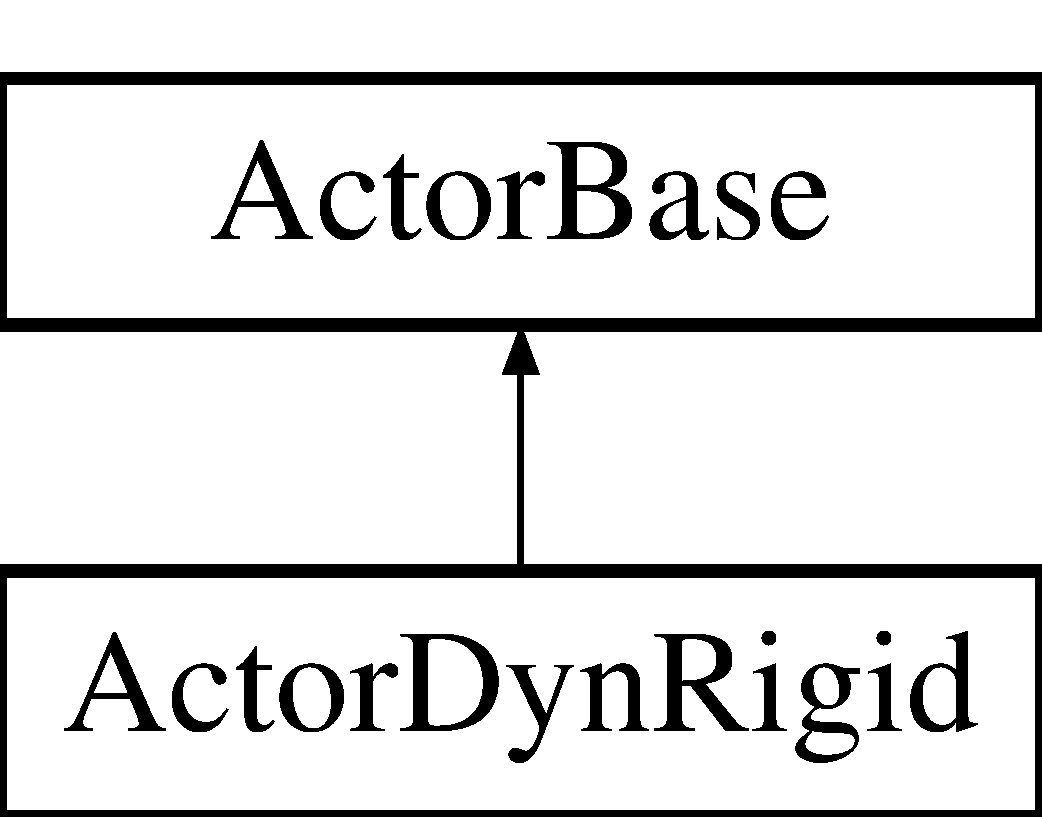
\includegraphics[height=2cm]{d4/d0e/classActorDynRigid}
\end{center}
\end{figure}
\subsection*{Public Member Functions}
\begin{DoxyCompactItemize}
\item 
\hyperlink{classActorDynRigid_a1402924eddf33a4789e3c3f68bbf6c98}{ActorDynRigid} (PhysReal mass, PhysString name, PhysString file, PhysString group, \hyperlink{classPhysWorld}{PhysWorld} $\ast$World)
\begin{DoxyCompactList}\small\item\em Descriptive constructor. \item\end{DoxyCompactList}\item 
virtual \hyperlink{classActorDynRigid_a3a5504a2ce11f1e95d29a6e431c0c2aa}{$\sim$ActorDynRigid} ()
\begin{DoxyCompactList}\small\item\em Destructor. \item\end{DoxyCompactList}\item 
void \hyperlink{classActorDynRigid_adbfe8a19f8aafe7928d9896c37821059}{CreateShapeFromMesh} ()
\begin{DoxyCompactList}\small\item\em Creates a collision shape from mesh file. \item\end{DoxyCompactList}\end{DoxyCompactItemize}
\subsection*{Protected Member Functions}
\begin{DoxyCompactItemize}
\item 
void \hyperlink{classActorDynRigid_a93052967ae8e6bebb810a5303ebc2a48}{CreateRigidObject} (PhysReal pmass)
\begin{DoxyCompactList}\small\item\em Creates a rigid object for the actor. \item\end{DoxyCompactList}\item 
void \hyperlink{classActorDynRigid_a45c054918362b86d829398384e316ed8}{AddObjectToWorld} (\hyperlink{classPhysWorld}{PhysWorld} $\ast$TargetWorld, btSoftRigidDynamicsWorld $\ast$World)
\begin{DoxyCompactList}\small\item\em Adds the actor to the physics world. \item\end{DoxyCompactList}\item 
virtual void \hyperlink{classActorDynRigid_a3f0720ca18d04a1084207d474c3d7834}{SetBulletLocation} (\hyperlink{classPhysVector3}{PhysVector3} Location)
\begin{DoxyCompactList}\small\item\em Sets the location of the physics body. \item\end{DoxyCompactList}\item 
virtual void \hyperlink{classActorDynRigid_ae471894081ae956dd79844a2f14fb1d9}{SetBulletOrientation} (\hyperlink{classPhysQuaternion}{PhysQuaternion} Rotation)
\begin{DoxyCompactList}\small\item\em Sets the orientation of the physics body. \item\end{DoxyCompactList}\end{DoxyCompactItemize}
\subsection*{Protected Attributes}
\begin{DoxyCompactItemize}
\item 
\hypertarget{classActorDynRigid_a83a6cb758304431043c6bfa05b47ecb2}{
btRigidBody $\ast$ {\bfseries physrigidbody}}
\label{d4/d0e/classActorDynRigid_a83a6cb758304431043c6bfa05b47ecb2}

\end{DoxyCompactItemize}


\subsection{Detailed Description}
This is the actor class for Dynamic Rigid Objects. This class should be used to make any rigid object that can be moved as a result of force. Most objects will fall into this catagory. A few examples of a Rigid Object: Boxes, Car Frames, Chairs, etc. For Semi Rigid bodies that are deformable, like jello, it is better to use \hyperlink{classActorDynSoft}{ActorDynSoft}. 

Definition at line 205 of file physactor.h.

\subsection{Constructor \& Destructor Documentation}
\hypertarget{classActorDynRigid_a1402924eddf33a4789e3c3f68bbf6c98}{
\index{ActorDynRigid@{ActorDynRigid}!ActorDynRigid@{ActorDynRigid}}
\index{ActorDynRigid@{ActorDynRigid}!ActorDynRigid@{ActorDynRigid}}
\subsubsection[{ActorDynRigid}]{\setlength{\rightskip}{0pt plus 5cm}ActorDynRigid::ActorDynRigid (PhysReal {\em mass}, \/  PhysString {\em name}, \/  PhysString {\em file}, \/  PhysString {\em group}, \/  {\bf PhysWorld} $\ast$ {\em World})}}
\label{d4/d0e/classActorDynRigid_a1402924eddf33a4789e3c3f68bbf6c98}


Descriptive constructor. This constructor contains the basic information needed to make a Rigid Object. \par
 This class inherits from \hyperlink{classActorBase}{ActorBase}. 
\begin{DoxyParams}{Parameters}
\item[{\em Mass}]The mass the object will have in the \hyperlink{classPhysWorld}{PhysWorld}. \item[{\em Name}]The name of the actor. \item[{\em File}]The 3d mesh file that contains the 3d model the actor will use. \item[{\em Group}]The resource group where the 3d mesh and other related files can be found. \item[{\em World}]Pointer to the \hyperlink{classPhysWorld}{PhysWorld} this object will be added to. \end{DoxyParams}


Definition at line 269 of file physactor.cpp.\hypertarget{classActorDynRigid_a3a5504a2ce11f1e95d29a6e431c0c2aa}{
\index{ActorDynRigid@{ActorDynRigid}!$\sim$ActorDynRigid@{$\sim$ActorDynRigid}}
\index{$\sim$ActorDynRigid@{$\sim$ActorDynRigid}!ActorDynRigid@{ActorDynRigid}}
\subsubsection[{$\sim$ActorDynRigid}]{\setlength{\rightskip}{0pt plus 5cm}ActorDynRigid::$\sim$ActorDynRigid ()\hspace{0.3cm}{\ttfamily  \mbox{[}virtual\mbox{]}}}}
\label{d4/d0e/classActorDynRigid_a3a5504a2ce11f1e95d29a6e431c0c2aa}


Destructor. The class destructor. 

Definition at line 274 of file physactor.cpp.

\subsection{Member Function Documentation}
\hypertarget{classActorDynRigid_a45c054918362b86d829398384e316ed8}{
\index{ActorDynRigid@{ActorDynRigid}!AddObjectToWorld@{AddObjectToWorld}}
\index{AddObjectToWorld@{AddObjectToWorld}!ActorDynRigid@{ActorDynRigid}}
\subsubsection[{AddObjectToWorld}]{\setlength{\rightskip}{0pt plus 5cm}void ActorDynRigid::AddObjectToWorld ({\bf PhysWorld} $\ast$ {\em TargetWorld}, \/  btSoftRigidDynamicsWorld $\ast$ {\em World})\hspace{0.3cm}{\ttfamily  \mbox{[}protected, virtual\mbox{]}}}}
\label{d4/d0e/classActorDynRigid_a45c054918362b86d829398384e316ed8}


Adds the actor to the physics world. Adds the actor to the physics world. \par
 This is automaticly called by the PhysWorlds AddActor function and shouldn't be called manually. 
\begin{DoxyParams}{Parameters}
\item[{\em TargetWorld}]Pointer to the \hyperlink{classPhysWorld}{PhysWorld} class. \item[{\em World}]Pointer to the physics world. \end{DoxyParams}


Implements \hyperlink{classActorBase_a1af82a2ed960fd114518fdf84d5ff146}{ActorBase}.

Definition at line 285 of file physactor.cpp.\hypertarget{classActorDynRigid_a93052967ae8e6bebb810a5303ebc2a48}{
\index{ActorDynRigid@{ActorDynRigid}!CreateRigidObject@{CreateRigidObject}}
\index{CreateRigidObject@{CreateRigidObject}!ActorDynRigid@{ActorDynRigid}}
\subsubsection[{CreateRigidObject}]{\setlength{\rightskip}{0pt plus 5cm}void ActorDynRigid::CreateRigidObject (PhysReal {\em pmass})\hspace{0.3cm}{\ttfamily  \mbox{[}protected\mbox{]}}}}
\label{d4/d0e/classActorDynRigid_a93052967ae8e6bebb810a5303ebc2a48}


Creates a rigid object for the actor. Creates a rigid object to be placed in the physics world later. \par
 This is automaticly called by the Constructor and shouldn't be called manually. 
\begin{DoxyParams}{Parameters}
\item[{\em PMass}]\char`\"{}PhysReal Mass\char`\"{} The mass of the object. \end{DoxyParams}


Definition at line 279 of file physactor.cpp.\hypertarget{classActorDynRigid_adbfe8a19f8aafe7928d9896c37821059}{
\index{ActorDynRigid@{ActorDynRigid}!CreateShapeFromMesh@{CreateShapeFromMesh}}
\index{CreateShapeFromMesh@{CreateShapeFromMesh}!ActorDynRigid@{ActorDynRigid}}
\subsubsection[{CreateShapeFromMesh}]{\setlength{\rightskip}{0pt plus 5cm}void ActorDynRigid::CreateShapeFromMesh ()}}
\label{d4/d0e/classActorDynRigid_adbfe8a19f8aafe7928d9896c37821059}


Creates a collision shape from mesh file. This function will read the location of every verticy in the mesh file and use that to construct a triangle mesh shape and attach it to this objects collision shape. 

Definition at line 303 of file physactor.cpp.\hypertarget{classActorDynRigid_a3f0720ca18d04a1084207d474c3d7834}{
\index{ActorDynRigid@{ActorDynRigid}!SetBulletLocation@{SetBulletLocation}}
\index{SetBulletLocation@{SetBulletLocation}!ActorDynRigid@{ActorDynRigid}}
\subsubsection[{SetBulletLocation}]{\setlength{\rightskip}{0pt plus 5cm}void ActorDynRigid::SetBulletLocation ({\bf PhysVector3} {\em Location})\hspace{0.3cm}{\ttfamily  \mbox{[}protected, virtual\mbox{]}}}}
\label{d4/d0e/classActorDynRigid_a3f0720ca18d04a1084207d474c3d7834}


Sets the location of the physics body. This will take a \hyperlink{classPhysVector3}{PhysVector3} and set the location of the actor within the physics world. \par
 This function is called on by the SetLocation function, and shouldn't be called manually. 

Reimplemented from \hyperlink{classActorBase_af64a57138bbd32c52581a5c8d0d29a76}{ActorBase}.

Definition at line 291 of file physactor.cpp.\hypertarget{classActorDynRigid_ae471894081ae956dd79844a2f14fb1d9}{
\index{ActorDynRigid@{ActorDynRigid}!SetBulletOrientation@{SetBulletOrientation}}
\index{SetBulletOrientation@{SetBulletOrientation}!ActorDynRigid@{ActorDynRigid}}
\subsubsection[{SetBulletOrientation}]{\setlength{\rightskip}{0pt plus 5cm}void ActorDynRigid::SetBulletOrientation ({\bf PhysQuaternion} {\em Rotation})\hspace{0.3cm}{\ttfamily  \mbox{[}protected, virtual\mbox{]}}}}
\label{d4/d0e/classActorDynRigid_ae471894081ae956dd79844a2f14fb1d9}


Sets the orientation of the physics body. This will take a \hyperlink{classPhysQuaternion}{PhysQuaternion} and set the orientation of the actor within the physics world. \par
 This function is called on by the SetOrientation function, and shouldn't be called manually. 
\begin{DoxyParams}{Parameters}
\item[{\em Rotation}]The quaternion representing the rotation of the actor. \end{DoxyParams}


Reimplemented from \hyperlink{classActorBase_adf817bd5a7c562f31f6724a06a3a0f79}{ActorBase}.

Definition at line 297 of file physactor.cpp.

The documentation for this class was generated from the following files:\begin{DoxyCompactItemize}
\item 
physactor.h\item 
physactor.cpp\end{DoxyCompactItemize}

\hypertarget{classActorDynSoft}{
\section{ActorDynSoft Class Reference}
\label{dc/de0/classActorDynSoft}\index{ActorDynSoft@{ActorDynSoft}}
}


This is the actor class for Dynamic Soft Objects.  


{\ttfamily \#include $<$physactor.h$>$}Inheritance diagram for ActorDynSoft::\begin{figure}[H]
\begin{center}
\leavevmode
\includegraphics[height=2cm]{dc/de0/classActorDynSoft}
\end{center}
\end{figure}
\subsection*{Public Member Functions}
\begin{DoxyCompactItemize}
\item 
virtual \hyperlink{classActorDynSoft_a8d2941aee946c14ce616d4d856ddf758}{$\sim$ActorDynSoft} ()
\begin{DoxyCompactList}\small\item\em Destructor. \item\end{DoxyCompactList}\item 
void \hyperlink{classActorDynSoft_a979620b4ac447eb9875fb769d61a8092}{CreateShapeFromMesh} ()
\begin{DoxyCompactList}\small\item\em Creates a collision shape from mesh file. \item\end{DoxyCompactList}\end{DoxyCompactItemize}
\subsection*{Protected Member Functions}
\begin{DoxyCompactItemize}
\item 
void \hyperlink{classActorDynSoft_a249bc0621b1d55ea0a9c7787605078d6}{CreateSoftObject} ()
\begin{DoxyCompactList}\small\item\em Creates a soft object for the actor. \item\end{DoxyCompactList}\item 
void \hyperlink{classActorDynSoft_ab56b961689401e16962d653b977e5fd6}{AddObjectToWorld} (\hyperlink{classPhysWorld}{PhysWorld} $\ast$TargetWorld, btSoftRigidDynamicsWorld $\ast$World)
\begin{DoxyCompactList}\small\item\em Adds the actor to the physics world. \item\end{DoxyCompactList}\item 
virtual void \hyperlink{classActorDynSoft_aaf548f7849f59956c10d79420efafffb}{SetBulletLocation} (\hyperlink{classPhysVector3}{PhysVector3} Location)
\begin{DoxyCompactList}\small\item\em Sets the location of the physics body. \item\end{DoxyCompactList}\item 
virtual void \hyperlink{classActorDynSoft_abbb2c795bd07b014239f157b440bc53d}{SetBulletOrientation} (\hyperlink{classPhysQuaternion}{PhysQuaternion} Rotation)
\begin{DoxyCompactList}\small\item\em Sets the orientation of the physics body. \item\end{DoxyCompactList}\end{DoxyCompactItemize}
\subsection*{Protected Attributes}
\begin{DoxyCompactItemize}
\item 
\hypertarget{classActorDynSoft_a59e1b9ae866bfd9af4bc2eebaf11a2d9}{
btSoftBody $\ast$ {\bfseries physsoftbody}}
\label{dc/de0/classActorDynSoft_a59e1b9ae866bfd9af4bc2eebaf11a2d9}

\end{DoxyCompactItemize}


\subsection{Detailed Description}
This is the actor class for Dynamic Soft Objects. This class should be used to make any soft object that, like \hyperlink{classActorDynRigid}{ActorDynRigid}, can be moved or manipulated as a result of force. Examples of soft objects are: Paper, Rope, and Cloth. Semi Rigid bodies that are still somewhat deformable, like Jello, should be made as a soft object. 

Definition at line 259 of file physactor.h.

\subsection{Constructor \& Destructor Documentation}
\hypertarget{classActorDynSoft_a8d2941aee946c14ce616d4d856ddf758}{
\index{ActorDynSoft@{ActorDynSoft}!$\sim$ActorDynSoft@{$\sim$ActorDynSoft}}
\index{$\sim$ActorDynSoft@{$\sim$ActorDynSoft}!ActorDynSoft@{ActorDynSoft}}
\subsubsection[{$\sim$ActorDynSoft}]{\setlength{\rightskip}{0pt plus 5cm}ActorDynSoft::$\sim$ActorDynSoft ()\hspace{0.3cm}{\ttfamily  \mbox{[}virtual\mbox{]}}}}
\label{dc/de0/classActorDynSoft_a8d2941aee946c14ce616d4d856ddf758}


Destructor. The class destructor. 

Definition at line 316 of file physactor.cpp.

\subsection{Member Function Documentation}
\hypertarget{classActorDynSoft_ab56b961689401e16962d653b977e5fd6}{
\index{ActorDynSoft@{ActorDynSoft}!AddObjectToWorld@{AddObjectToWorld}}
\index{AddObjectToWorld@{AddObjectToWorld}!ActorDynSoft@{ActorDynSoft}}
\subsubsection[{AddObjectToWorld}]{\setlength{\rightskip}{0pt plus 5cm}void ActorDynSoft::AddObjectToWorld ({\bf PhysWorld} $\ast$ {\em TargetWorld}, \/  btSoftRigidDynamicsWorld $\ast$ {\em World})\hspace{0.3cm}{\ttfamily  \mbox{[}protected, virtual\mbox{]}}}}
\label{dc/de0/classActorDynSoft_ab56b961689401e16962d653b977e5fd6}


Adds the actor to the physics world. Adds the actor to the physics world. \par
 This is automaticly called by the PhysWorlds AddActor function and shouldn't be called manually. 
\begin{DoxyParams}{Parameters}
\item[{\em TargetWorld}]Pointer to the \hyperlink{classPhysWorld}{PhysWorld} class. \item[{\em World}]Pointer to the physics world. \end{DoxyParams}


Implements \hyperlink{classActorBase_a1af82a2ed960fd114518fdf84d5ff146}{ActorBase}.

Definition at line 324 of file physactor.cpp.\hypertarget{classActorDynSoft_a979620b4ac447eb9875fb769d61a8092}{
\index{ActorDynSoft@{ActorDynSoft}!CreateShapeFromMesh@{CreateShapeFromMesh}}
\index{CreateShapeFromMesh@{CreateShapeFromMesh}!ActorDynSoft@{ActorDynSoft}}
\subsubsection[{CreateShapeFromMesh}]{\setlength{\rightskip}{0pt plus 5cm}void ActorDynSoft::CreateShapeFromMesh ()}}
\label{dc/de0/classActorDynSoft_a979620b4ac447eb9875fb769d61a8092}


Creates a collision shape from mesh file. This function will read the location of every verticy in the mesh file and use that to construct a triangle mesh shape and attach it to this objects collision shape. 

Definition at line 341 of file physactor.cpp.\hypertarget{classActorDynSoft_a249bc0621b1d55ea0a9c7787605078d6}{
\index{ActorDynSoft@{ActorDynSoft}!CreateSoftObject@{CreateSoftObject}}
\index{CreateSoftObject@{CreateSoftObject}!ActorDynSoft@{ActorDynSoft}}
\subsubsection[{CreateSoftObject}]{\setlength{\rightskip}{0pt plus 5cm}void ActorDynSoft::CreateSoftObject ()\hspace{0.3cm}{\ttfamily  \mbox{[}protected\mbox{]}}}}
\label{dc/de0/classActorDynSoft_a249bc0621b1d55ea0a9c7787605078d6}


Creates a soft object for the actor. Creates a soft object to be placed in the physics world later. \par
 This is automaticly called by the Constructor and shouldn't be called manually. 

Definition at line 320 of file physactor.cpp.\hypertarget{classActorDynSoft_aaf548f7849f59956c10d79420efafffb}{
\index{ActorDynSoft@{ActorDynSoft}!SetBulletLocation@{SetBulletLocation}}
\index{SetBulletLocation@{SetBulletLocation}!ActorDynSoft@{ActorDynSoft}}
\subsubsection[{SetBulletLocation}]{\setlength{\rightskip}{0pt plus 5cm}void ActorDynSoft::SetBulletLocation ({\bf PhysVector3} {\em Location})\hspace{0.3cm}{\ttfamily  \mbox{[}protected, virtual\mbox{]}}}}
\label{dc/de0/classActorDynSoft_aaf548f7849f59956c10d79420efafffb}


Sets the location of the physics body. This will take a \hyperlink{classPhysVector3}{PhysVector3} and set the location of the actor within the physics world. \par
 This function is called on by the SetLocation function, and shouldn't be called manually. 

Reimplemented from \hyperlink{classActorBase_af64a57138bbd32c52581a5c8d0d29a76}{ActorBase}.

Definition at line 329 of file physactor.cpp.\hypertarget{classActorDynSoft_abbb2c795bd07b014239f157b440bc53d}{
\index{ActorDynSoft@{ActorDynSoft}!SetBulletOrientation@{SetBulletOrientation}}
\index{SetBulletOrientation@{SetBulletOrientation}!ActorDynSoft@{ActorDynSoft}}
\subsubsection[{SetBulletOrientation}]{\setlength{\rightskip}{0pt plus 5cm}void ActorDynSoft::SetBulletOrientation ({\bf PhysQuaternion} {\em Rotation})\hspace{0.3cm}{\ttfamily  \mbox{[}protected, virtual\mbox{]}}}}
\label{dc/de0/classActorDynSoft_abbb2c795bd07b014239f157b440bc53d}


Sets the orientation of the physics body. This will take a \hyperlink{classPhysQuaternion}{PhysQuaternion} and set the orientation of the actor within the physics world. \par
 This function is called on by the SetOrientation function, and shouldn't be called manually. 
\begin{DoxyParams}{Parameters}
\item[{\em Rotation}]The quaternion representing the rotation of the actor. \end{DoxyParams}


Reimplemented from \hyperlink{classActorBase_adf817bd5a7c562f31f6724a06a3a0f79}{ActorBase}.

Definition at line 335 of file physactor.cpp.

The documentation for this class was generated from the following files:\begin{DoxyCompactItemize}
\item 
physactor.h\item 
physactor.cpp\end{DoxyCompactItemize}

\hypertarget{classActorSta}{
\section{ActorSta Class Reference}
\label{d3/daf/classActorSta}\index{ActorSta@{ActorSta}}
}
Inheritance diagram for ActorSta::\begin{figure}[H]
\begin{center}
\leavevmode
\includegraphics[height=2cm]{d3/daf/classActorSta}
\end{center}
\end{figure}
\subsection*{Public Member Functions}
\begin{DoxyCompactItemize}
\item 
\hypertarget{classActorSta_a970ee3677eca8f69f6d25684d72c6c8c}{
{\bfseries ActorSta} (PhysString name, PhysString file)}
\label{d3/daf/classActorSta_a970ee3677eca8f69f6d25684d72c6c8c}

\item 
\hypertarget{classActorSta_ae856b69de748541606649d21d2e6c270}{
void {\bfseries CreateRigidObject} ()}
\label{d3/daf/classActorSta_ae856b69de748541606649d21d2e6c270}

\end{DoxyCompactItemize}
\subsection*{Protected Member Functions}
\begin{DoxyCompactItemize}
\item 
\hypertarget{classActorSta_a8d403fae36b366368982a4453d740a27}{
void {\bfseries AddObjectToWorld} (\hyperlink{classPhysWorld}{PhysWorld} $\ast$TargetWorld, btDiscreteDynamicsWorld $\ast$TargetPhysicsWorld)}
\label{d3/daf/classActorSta_a8d403fae36b366368982a4453d740a27}

\end{DoxyCompactItemize}
\subsection*{Protected Attributes}
\begin{DoxyCompactItemize}
\item 
\hypertarget{classActorSta_ad12363fc4cd60d6cdd5e3c6d36d96f20}{
btRigidBody $\ast$ {\bfseries physrigidbody}}
\label{d3/daf/classActorSta_ad12363fc4cd60d6cdd5e3c6d36d96f20}

\end{DoxyCompactItemize}


\subsection{Detailed Description}


Definition at line 135 of file physactor.h.

The documentation for this class was generated from the following files:\begin{DoxyCompactItemize}
\item 
physactor.h\item 
physactor.cpp\end{DoxyCompactItemize}

\hypertarget{classMetaCode}{
\section{MetaCode Class Reference}
\label{d7/d72/classMetaCode}\index{MetaCode@{MetaCode}}
}
\subsection*{Public Member Functions}
\begin{DoxyCompactItemize}
\item 
\hypertarget{classMetaCode_a76bba215580768ab22c505ea18b2ec6d}{
{\bfseries MetaCode} (int MetaValue\_\-, short unsigned int ID\_\-, InputCode Code\_\-)}
\label{d7/d72/classMetaCode_a76bba215580768ab22c505ea18b2ec6d}

\item 
\hypertarget{classMetaCode_ad0a739796fa1de2991c196d8ee7b19b2}{
{\bfseries MetaCode} (RawEvent \_\-RawEvent)}
\label{d7/d72/classMetaCode_ad0a739796fa1de2991c196d8ee7b19b2}

\item 
\hypertarget{classMetaCode_a9438d04aa38086baa1c5ccd79510c0fb}{
InputCode {\bfseries GetCode} ()}
\label{d7/d72/classMetaCode_a9438d04aa38086baa1c5ccd79510c0fb}

\item 
\hypertarget{classMetaCode_a24f0c5469a12ccc59fcf3b830e6cfc27}{
void {\bfseries SetCode} (InputCode Code\_\-)}
\label{d7/d72/classMetaCode_a24f0c5469a12ccc59fcf3b830e6cfc27}

\item 
\hypertarget{classMetaCode_a6a33ef9b7e2414ecfd97aadb14eca2de}{
int {\bfseries GetMetaValue} ()}
\label{d7/d72/classMetaCode_a6a33ef9b7e2414ecfd97aadb14eca2de}

\item 
\hypertarget{classMetaCode_a308404d4eb64627d02ab41dd5029c9c8}{
void {\bfseries SetMetaValue} (int MetaValue\_\-)}
\label{d7/d72/classMetaCode_a308404d4eb64627d02ab41dd5029c9c8}

\item 
\hypertarget{classMetaCode_a4556130570fdc8bf531be7f15519fafe}{
short unsigned int {\bfseries GetID} ()}
\label{d7/d72/classMetaCode_a4556130570fdc8bf531be7f15519fafe}

\item 
\hypertarget{classMetaCode_ae39bd781449cc01d7bce48c1e9da089d}{
void {\bfseries SetID} (short unsigned int ID\_\-)}
\label{d7/d72/classMetaCode_ae39bd781449cc01d7bce48c1e9da089d}

\item 
\hypertarget{classMetaCode_a296b774682a9326494e0c2d1b357ec2a}{
bool {\bfseries operator==} (const \hyperlink{classMetaCode}{MetaCode} \&other) const }
\label{d7/d72/classMetaCode_a296b774682a9326494e0c2d1b357ec2a}

\end{DoxyCompactItemize}


\subsection{Detailed Description}


Definition at line 330 of file physeventuserinput.h.

The documentation for this class was generated from the following files:\begin{DoxyCompactItemize}
\item 
physeventuserinput.h\item 
physeventuserinput.cpp\end{DoxyCompactItemize}

\hypertarget{classPhysEvent}{
\section{PhysEvent Class Reference}
\label{d9/dc2/classPhysEvent}\index{PhysEvent@{PhysEvent}}
}
Inheritance diagram for PhysEvent::\begin{figure}[H]
\begin{center}
\leavevmode
\includegraphics[height=2cm]{d9/dc2/classPhysEvent}
\end{center}
\end{figure}
\subsection*{Public Types}
\begin{DoxyCompactItemize}
\item 
enum {\bfseries EventType} \{ \par
{\bfseries RenderTime}, 
{\bfseries UserInput}, 
{\bfseries QuitMessage}, 
{\bfseries SystemMessage}, 
\par
{\bfseries Other}
 \}
\end{DoxyCompactItemize}
\subsection*{Public Member Functions}
\begin{DoxyCompactItemize}
\item 
\hypertarget{classPhysEvent_aca0328653fffcc9b1072b290074f29c0}{
virtual PhysEvent::EventType {\bfseries getEventType} () const =0}
\label{d9/dc2/classPhysEvent_aca0328653fffcc9b1072b290074f29c0}

\end{DoxyCompactItemize}


\subsection{Detailed Description}


Definition at line 53 of file physevent.h.

The documentation for this class was generated from the following file:\begin{DoxyCompactItemize}
\item 
physevent.h\end{DoxyCompactItemize}

\hypertarget{classPhysEventManager}{
\section{PhysEventManager Class Reference}
\label{d5/dd7/classPhysEventManager}\index{PhysEventManager@{PhysEventManager}}
}


This is a container for Events and facilitates the transfer of data.  


{\ttfamily \#include $<$physeventmanager.h$>$}\subsection*{Public Member Functions}
\begin{DoxyCompactItemize}
\item 
\hyperlink{classPhysEventManager_a1355f36d99de303cec6f3b27cadaa9ff}{PhysEventManager} (\hyperlink{classPhysWorld}{PhysWorld} $\ast$ParentWorld\_\-)
\begin{DoxyCompactList}\small\item\em Default constructor. \item\end{DoxyCompactList}\item 
unsigned int \hyperlink{classPhysEventManager_ab14d238e7abe9919be8e2d9eef388b64}{GetRemainingEventCount} ()
\begin{DoxyCompactList}\small\item\em Gets a count of events. \item\end{DoxyCompactList}\item 
\hyperlink{classPhysEvent}{PhysEvent} $\ast$ \hyperlink{classPhysEventManager_a6de94bc6c23dcbd7e15785cadee2e80b}{GetNextEvent} ()
\begin{DoxyCompactList}\small\item\em Return a pointer to the Next event. \item\end{DoxyCompactList}\item 
\hyperlink{classPhysEvent}{PhysEvent} $\ast$ \hyperlink{classPhysEventManager_a3122b32172326ac32cfecc828b820977}{PopNextEvent} ()
\begin{DoxyCompactList}\small\item\em Return a pointer to the Next event, and removes the Event from storage. \item\end{DoxyCompactList}\item 
void \hyperlink{classPhysEventManager_ad040054bd9018ff0fd27ad78ec1e87fa}{RemoveNextEvent} ()
\begin{DoxyCompactList}\small\item\em Removes an Event From the que without looking at it. \item\end{DoxyCompactList}\item 
void \hyperlink{classPhysEventManager_a7c9bb46b17f6d9245817a402dc6a2f6f}{AddEvent} (\hyperlink{classPhysEvent}{PhysEvent} $\ast$EventToAdd)
\begin{DoxyCompactList}\small\item\em Adds an event of any kind to the end of the Event Queue. \item\end{DoxyCompactList}\item 
\hypertarget{classPhysEventManager_a34b4b8d35fee0f593fbb32b83843abba}{
void {\bfseries UpdateEvents} ()}
\label{d5/dd7/classPhysEventManager_a34b4b8d35fee0f593fbb32b83843abba}

\item 
\hypertarget{classPhysEventManager_adcdeb687464f00252e1c4052d4b9304e}{
void {\bfseries UpdateSystemEvents} ()}
\label{d5/dd7/classPhysEventManager_adcdeb687464f00252e1c4052d4b9304e}

\item 
\hypertarget{classPhysEventManager_a99f2350628caf751e156107d57646030}{
void {\bfseries UpdateUserInputEvents} ()}
\label{d5/dd7/classPhysEventManager_a99f2350628caf751e156107d57646030}

\item 
\hyperlink{classPhysEventRenderTime}{PhysEventRenderTime} $\ast$ \hyperlink{classPhysEventManager_a1f2d0506ce816176913e5bdfaa9fd724}{GetNextRenderTimeEvent} ()
\begin{DoxyCompactList}\small\item\em Returns a pointer to the Next Rendertime event. \item\end{DoxyCompactList}\item 
\hyperlink{classPhysEventRenderTime}{PhysEventRenderTime} $\ast$ \hyperlink{classPhysEventManager_ad627925363fdbcff98e0faef204e81e2}{PopNextRenderTimeEvent} ()
\begin{DoxyCompactList}\small\item\em Returns a pointer to the Next Rendertime event and removes it from the Que. \item\end{DoxyCompactList}\item 
void \hyperlink{classPhysEventManager_a56acc075e743921e27284c023b3298ce}{RemoveNextRenderTimeEvent} ()
\begin{DoxyCompactList}\small\item\em Removes the First Rendertime Event From the que without looking at it. \item\end{DoxyCompactList}\item 
\hyperlink{classPhysEventUserInput}{PhysEventUserInput} $\ast$ \hyperlink{classPhysEventManager_a4874a9b1138d2351bf28e527a66c02b8}{GetNextUserInputEvent} ()
\begin{DoxyCompactList}\small\item\em Returns a pointer to the Next User Input event. \item\end{DoxyCompactList}\item 
\hyperlink{classPhysEventUserInput}{PhysEventUserInput} $\ast$ \hyperlink{classPhysEventManager_ad6612a6e1c728941e2c467e7f136ca51}{PopNextUserInputEvent} ()
\begin{DoxyCompactList}\small\item\em Returns a pointer to the Next User Input event and removes it from the Que. \item\end{DoxyCompactList}\item 
void \hyperlink{classPhysEventManager_a9c6f5296c9961fa469ebe06d7599283a}{RemoveNextUserInputEvent} ()
\begin{DoxyCompactList}\small\item\em Removes the First User Input Event From the que without looking at it. \item\end{DoxyCompactList}\item 
\hypertarget{classPhysEventManager_a61aa2ee266536d45fec2be0487f77940}{
\hyperlink{classEventQuit}{EventQuit} $\ast$ {\bfseries GetNextQuitEvent} ()}
\label{d5/dd7/classPhysEventManager_a61aa2ee266536d45fec2be0487f77940}

\item 
\hypertarget{classPhysEventManager_a1def6dcacc5dd8a0d55dd2d47fe89a1c}{
\hyperlink{classEventQuit}{EventQuit} $\ast$ {\bfseries PopNextQuitEvent} ()}
\label{d5/dd7/classPhysEventManager_a1def6dcacc5dd8a0d55dd2d47fe89a1c}

\item 
\hypertarget{classPhysEventManager_accdd3b4047b05b721f77ca68e016baf5}{
void {\bfseries RemoveNextQuitEvent} ()}
\label{d5/dd7/classPhysEventManager_accdd3b4047b05b721f77ca68e016baf5}

\item 
\hyperlink{classPhysEvent}{PhysEvent} $\ast$ \hyperlink{classPhysEventManager_a56e45572c2fb84131f7d55c060c7ac21}{GetNextSpecificEvent} (PhysEvent::EventType SpecificType)
\begin{DoxyCompactList}\small\item\em Returns a pointer to the Next kind event of the Specified type. \item\end{DoxyCompactList}\item 
\hyperlink{classPhysEvent}{PhysEvent} $\ast$ \hyperlink{classPhysEventManager_abce156f7ad7ab145b8b05740b48e6073}{PopNextSpecificEvent} (PhysEvent::EventType SpecificType)
\begin{DoxyCompactList}\small\item\em Returns a pointer to the Next kind event of the Specified type, and removes it from the Que. \item\end{DoxyCompactList}\item 
void \hyperlink{classPhysEventManager_a2d0c21e369d16cd2de97eb4c69003323}{RemoveNextSpecificEvent} (PhysEvent::EventType SpecificType)
\begin{DoxyCompactList}\small\item\em Returns a pointer to the Next kind event of the Specified type, and removes it from the Que. \item\end{DoxyCompactList}\item 
void \hyperlink{classPhysEventManager_a1e99385441c5377a741561db581ef3ae}{AddPollingCheck} (const \hyperlink{classMetaCode}{MetaCode} \&InputToTryPolling)
\begin{DoxyCompactList}\small\item\em Generates extra events each iteration of the main loop, based on user input polling. \item\end{DoxyCompactList}\item 
void \hyperlink{classPhysEventManager_af81bf9a5f081f44a6cd91fdd19d4a42a}{RemovePollingCheck} (const \hyperlink{classMetaCode}{MetaCode} \&InputToStopPolling)
\begin{DoxyCompactList}\small\item\em Removes Events from the list(s) of what needs to be polled. \item\end{DoxyCompactList}\item 
\hyperlink{classPhysEventUserInput}{PhysEventUserInput} $\ast$ \hyperlink{classPhysEventManager_ac66ebe495e2a77d06803291711528db2}{PollForUserInputEvents} ()
\begin{DoxyCompactList}\small\item\em This activates the polling routines of the user input subsystems. \item\end{DoxyCompactList}\end{DoxyCompactItemize}


\subsection{Detailed Description}
This is a container for Events and facilitates the transfer of data. The Event Manager Exists to passed important information about Gamestate from where it is generated to where it is needed. It is the Game Developers option whether they want to grab events directly using the get functions that have filters, or if they want to get all the events at once from a central location and dispatch form there. \par
 Since all User input comes in the form of events, this is also where user input Polling and optional input sources like Joysticks are controlled from. \par
 All of these event are stored in an internal Queue and order is preserved. So the First item In will be the First Out (FIFO). This is not strictly a FIFO buffer, there are a number of functions for getting of managing specific kinds of events. Generally these 'Filtered' management functions Still return the first of those kinds of event. \begin{DoxyWarning}{Warning}
Delete pointers you get from this. Anything can create events and Put them here, and anything can get them out, This means the simple way to not cause memory leaks is to have the routines extracting the events delete the events. 

Currently this is not thread safe, even though it should be. 
\end{DoxyWarning}


Definition at line 83 of file physeventmanager.h.

\subsection{Constructor \& Destructor Documentation}
\hypertarget{classPhysEventManager_a1355f36d99de303cec6f3b27cadaa9ff}{
\index{PhysEventManager@{PhysEventManager}!PhysEventManager@{PhysEventManager}}
\index{PhysEventManager@{PhysEventManager}!PhysEventManager@{PhysEventManager}}
\subsubsection[{PhysEventManager}]{\setlength{\rightskip}{0pt plus 5cm}PhysEventManager::PhysEventManager ({\bf PhysWorld} $\ast$ {\em ParentWorld\_\-})}}
\label{d5/dd7/classPhysEventManager_a1355f36d99de303cec6f3b27cadaa9ff}


Default constructor. \begin{Desc}
\item[\hyperlink{todo__todo000006}{Todo}]TODO build a deconstructor that deletes all the events still int the queue \end{Desc}

\begin{DoxyParams}{Parameters}
\item[{\em ParentWorld\_\-}]A pointer to the world that this physworld is working with Primarily\end{DoxyParams}
This creates an empty PhysEventManger

\begin{Desc}
\item[\hyperlink{todo__todo000005}{Todo}]TODO: Make the \hyperlink{classPhysEventManager}{PhysEventManager} completely thread safe. IF this is completely thread safe, we can spawn numerous individual thread each accessing this and and the performance gain would almost scale directly with cpu core count increases. Look at boost scoped\_\-lock \end{Desc}


Definition at line 89 of file physeventmanager.cpp.

\subsection{Member Function Documentation}
\hypertarget{classPhysEventManager_a7c9bb46b17f6d9245817a402dc6a2f6f}{
\index{PhysEventManager@{PhysEventManager}!AddEvent@{AddEvent}}
\index{AddEvent@{AddEvent}!PhysEventManager@{PhysEventManager}}
\subsubsection[{AddEvent}]{\setlength{\rightskip}{0pt plus 5cm}void PhysEventManager::AddEvent ({\bf PhysEvent} $\ast$ {\em EventToAdd})}}
\label{d5/dd7/classPhysEventManager_a7c9bb46b17f6d9245817a402dc6a2f6f}


Adds an event of any kind to the end of the Event Queue. 
\begin{DoxyParams}{Parameters}
\item[{\em EventToAdd}]This is a pointer to an Event.\end{DoxyParams}
This adds the existing event to the Queue. Be careful this is not delete, and does not go out of scope. Deleting the Event is now the responsibilty of the code that pulls it out of Event Manager. 

Definition at line 130 of file physeventmanager.cpp.\hypertarget{classPhysEventManager_a1e99385441c5377a741561db581ef3ae}{
\index{PhysEventManager@{PhysEventManager}!AddPollingCheck@{AddPollingCheck}}
\index{AddPollingCheck@{AddPollingCheck}!PhysEventManager@{PhysEventManager}}
\subsubsection[{AddPollingCheck}]{\setlength{\rightskip}{0pt plus 5cm}void PhysEventManager::AddPollingCheck (const {\bf MetaCode} \& {\em InputToTryPolling})}}
\label{d5/dd7/classPhysEventManager_a1e99385441c5377a741561db581ef3ae}


Generates extra events each iteration of the main loop, based on user input polling. 
\begin{DoxyParams}{Parameters}
\item[{\em InputToTryPolling}]This accepts a \hyperlink{classMetaCode}{MetaCode} and will try to watch for occurences like this one\end{DoxyParams}
This will trigger the input system to generate an event (or add to an exiting event) when polling for the given kind of event. Each Iteration of the main loop there will be a \hyperlink{classPhysEventUserInput}{PhysEventUserInput} that created. That Event will Include all the normal metacodes for user input that happened, and it will also have a meta code for each time this function was called. The added metacode may be partialky ignored, the Metavalue is almost always ignored, and in a situation where the can only be one of a given input on a system, the ID is ignore and 0 is assumed. 
\begin{DoxyExceptions}{Exceptions}
\item[{\em Unsupported Polling Check on this Platform}]When the metacode passed cannot be polled on this platform \end{DoxyExceptions}


Definition at line 283 of file physeventmanager.cpp.\hypertarget{classPhysEventManager_a6de94bc6c23dcbd7e15785cadee2e80b}{
\index{PhysEventManager@{PhysEventManager}!GetNextEvent@{GetNextEvent}}
\index{GetNextEvent@{GetNextEvent}!PhysEventManager@{PhysEventManager}}
\subsubsection[{GetNextEvent}]{\setlength{\rightskip}{0pt plus 5cm}{\bf PhysEvent} $\ast$ PhysEventManager::GetNextEvent ()}}
\label{d5/dd7/classPhysEventManager_a6de94bc6c23dcbd7e15785cadee2e80b}


Return a pointer to the Next event. This returns a pointer to the next \hyperlink{classPhysEvent}{PhysEvent}. It is advisable to use this for performance reasons because it runs in constant time. However it does not return a specific kind of event, and must be cast in order to use the true content. This returns a pointer to 0 if there are no events in the que. \begin{DoxyReturn}{Returns}
A pointer to a \hyperlink{classPhysEvent}{PhysEvent}, that still needs to be removed from the event manager and deleted. 
\end{DoxyReturn}


Definition at line 104 of file physeventmanager.cpp.\hypertarget{classPhysEventManager_a1f2d0506ce816176913e5bdfaa9fd724}{
\index{PhysEventManager@{PhysEventManager}!GetNextRenderTimeEvent@{GetNextRenderTimeEvent}}
\index{GetNextRenderTimeEvent@{GetNextRenderTimeEvent}!PhysEventManager@{PhysEventManager}}
\subsubsection[{GetNextRenderTimeEvent}]{\setlength{\rightskip}{0pt plus 5cm}{\bf PhysEventRenderTime} $\ast$ PhysEventManager::GetNextRenderTimeEvent ()}}
\label{d5/dd7/classPhysEventManager_a1f2d0506ce816176913e5bdfaa9fd724}


Returns a pointer to the Next Rendertime event. This Filtered event management function returns a pointer to the next Rendertime event. It is inadvisable to use this for performance reasons becuase it runs in linear time relative to the amount of events. However, it will return an immediately usable pointer for case where an extreme level of performance is not required. This returns a pointer to 0 if there are no rendertime events in the que. \begin{DoxyReturn}{Returns}
A pointer to a \hyperlink{classPhysEventRenderTime}{PhysEventRenderTime}, that still needs to be removed from the event manager and deleted. 
\end{DoxyReturn}


Definition at line 226 of file physeventmanager.cpp.\hypertarget{classPhysEventManager_a56e45572c2fb84131f7d55c060c7ac21}{
\index{PhysEventManager@{PhysEventManager}!GetNextSpecificEvent@{GetNextSpecificEvent}}
\index{GetNextSpecificEvent@{GetNextSpecificEvent}!PhysEventManager@{PhysEventManager}}
\subsubsection[{GetNextSpecificEvent}]{\setlength{\rightskip}{0pt plus 5cm}{\bf PhysEvent} $\ast$ PhysEventManager::GetNextSpecificEvent (PhysEvent::EventType {\em SpecificType})}}
\label{d5/dd7/classPhysEventManager_a56e45572c2fb84131f7d55c060c7ac21}


Returns a pointer to the Next kind event of the Specified type. 
\begin{DoxyParams}{Parameters}
\item[{\em SpecificType}]This is a PhysEvent::EventType that defines the type you want this to work with\end{DoxyParams}
This and the other NextSpecificEvent functions are the core of the Event Filtering System. In general the other filtering functions call one of these and does very little work on their own. \par
 This performs a linear search starting with the oldest (first entered Events) and simply checks if it the of the correct type. Then this returns a pointer to the next event of the specified type, or returns a pointer to 0 if there are none of the correct pointers in the Que. It is inadvisable to use this for performance reasons becuase it runs in linear time relative to the amount of events. \begin{DoxyReturn}{Returns}
A pointer to a \hyperlink{classPhysEventUserInput}{PhysEventUserInput}, that still needs to be removed from the event manager and deleted. 
\end{DoxyReturn}


Definition at line 183 of file physeventmanager.cpp.\hypertarget{classPhysEventManager_a4874a9b1138d2351bf28e527a66c02b8}{
\index{PhysEventManager@{PhysEventManager}!GetNextUserInputEvent@{GetNextUserInputEvent}}
\index{GetNextUserInputEvent@{GetNextUserInputEvent}!PhysEventManager@{PhysEventManager}}
\subsubsection[{GetNextUserInputEvent}]{\setlength{\rightskip}{0pt plus 5cm}{\bf PhysEventUserInput} $\ast$ PhysEventManager::GetNextUserInputEvent ()}}
\label{d5/dd7/classPhysEventManager_a4874a9b1138d2351bf28e527a66c02b8}


Returns a pointer to the Next User Input event. This Filtered event management function returns a pointer to the next User Input event. It is inadvisable to use this for performance reasons becuase it runs in linear time relative to the amount of events. However, it will return an immediately usable pointer for case where an extreme level of performance is not required. This returns a pointer to 0 if there are no User Input events in the que. \begin{DoxyReturn}{Returns}
A pointer to a \hyperlink{classPhysEventUserInput}{PhysEventUserInput}, that still needs to be removed from the event manager and deleted. 
\end{DoxyReturn}


Definition at line 245 of file physeventmanager.cpp.\hypertarget{classPhysEventManager_ab14d238e7abe9919be8e2d9eef388b64}{
\index{PhysEventManager@{PhysEventManager}!GetRemainingEventCount@{GetRemainingEventCount}}
\index{GetRemainingEventCount@{GetRemainingEventCount}!PhysEventManager@{PhysEventManager}}
\subsubsection[{GetRemainingEventCount}]{\setlength{\rightskip}{0pt plus 5cm}unsigned int PhysEventManager::GetRemainingEventCount ()}}
\label{d5/dd7/classPhysEventManager_ab14d238e7abe9919be8e2d9eef388b64}


Gets a count of events. This returns a total count of all events stored in this \hyperlink{classPhysEventManager}{PhysEventManager}. \begin{DoxyReturn}{Returns}
This returns an unsigned integer with the amount of of total events 
\end{DoxyReturn}


Definition at line 99 of file physeventmanager.cpp.\hypertarget{classPhysEventManager_ac66ebe495e2a77d06803291711528db2}{
\index{PhysEventManager@{PhysEventManager}!PollForUserInputEvents@{PollForUserInputEvents}}
\index{PollForUserInputEvents@{PollForUserInputEvents}!PhysEventManager@{PhysEventManager}}
\subsubsection[{PollForUserInputEvents}]{\setlength{\rightskip}{0pt plus 5cm}{\bf PhysEventUserInput} $\ast$ PhysEventManager::PollForUserInputEvents ()}}
\label{d5/dd7/classPhysEventManager_ac66ebe495e2a77d06803291711528db2}


This activates the polling routines of the user input subsystems. This checks the current state of user input devices that have been added by \hyperlink{classPhysEventManager_a1e99385441c5377a741561db581ef3ae}{AddPollingCheck(const MetaCode \&InputToTryPolling)}. This is called automatically by main loop processing, but there is no harm in calling it several times. \begin{DoxyReturn}{Returns}
This returns a pointer to a \hyperlink{classPhysEventUserInput}{PhysEventUserInput} that contains the desired metacodes 
\end{DoxyReturn}


Definition at line 323 of file physeventmanager.cpp.\hypertarget{classPhysEventManager_a3122b32172326ac32cfecc828b820977}{
\index{PhysEventManager@{PhysEventManager}!PopNextEvent@{PopNextEvent}}
\index{PopNextEvent@{PopNextEvent}!PhysEventManager@{PhysEventManager}}
\subsubsection[{PopNextEvent}]{\setlength{\rightskip}{0pt plus 5cm}{\bf PhysEvent} $\ast$ PhysEventManager::PopNextEvent ()}}
\label{d5/dd7/classPhysEventManager_a3122b32172326ac32cfecc828b820977}


Return a pointer to the Next event, and removes the Event from storage. This functions just like GetNextEvent , except that it also removes the item from the internal storage of the \hyperlink{classPhysEventManager}{PhysEventManager}. This returns a pointer to 0 if there are no events in the que. \begin{DoxyReturn}{Returns}
A pointer to a \hyperlink{classPhysEvent}{PhysEvent}, that will need to be deleted once it has been used. 
\end{DoxyReturn}


Definition at line 114 of file physeventmanager.cpp.\hypertarget{classPhysEventManager_ad627925363fdbcff98e0faef204e81e2}{
\index{PhysEventManager@{PhysEventManager}!PopNextRenderTimeEvent@{PopNextRenderTimeEvent}}
\index{PopNextRenderTimeEvent@{PopNextRenderTimeEvent}!PhysEventManager@{PhysEventManager}}
\subsubsection[{PopNextRenderTimeEvent}]{\setlength{\rightskip}{0pt plus 5cm}{\bf PhysEventRenderTime} $\ast$ PhysEventManager::PopNextRenderTimeEvent ()}}
\label{d5/dd7/classPhysEventManager_ad627925363fdbcff98e0faef204e81e2}


Returns a pointer to the Next Rendertime event and removes it from the Que. This Filtered event management function returns a pointer to the next Rendertime event. It is inadvisable to use this for performance reasons becuase it runs in linear time relative to the amount of events. However, it will return an immediately usable pointer for case where an extreme level of performance is not required. This returns a pointer to 0 if there are no rendertime events in the que. This also removes the returned pointer form the Que. \begin{DoxyReturn}{Returns}
A pointer to a \hyperlink{classPhysEventRenderTime}{PhysEventRenderTime}, that still needs to be removed from the event manager and deleted. 
\end{DoxyReturn}


Definition at line 231 of file physeventmanager.cpp.\hypertarget{classPhysEventManager_abce156f7ad7ab145b8b05740b48e6073}{
\index{PhysEventManager@{PhysEventManager}!PopNextSpecificEvent@{PopNextSpecificEvent}}
\index{PopNextSpecificEvent@{PopNextSpecificEvent}!PhysEventManager@{PhysEventManager}}
\subsubsection[{PopNextSpecificEvent}]{\setlength{\rightskip}{0pt plus 5cm}{\bf PhysEvent} $\ast$ PhysEventManager::PopNextSpecificEvent (PhysEvent::EventType {\em SpecificType})}}
\label{d5/dd7/classPhysEventManager_abce156f7ad7ab145b8b05740b48e6073}


Returns a pointer to the Next kind event of the Specified type, and removes it from the Que. 
\begin{DoxyParams}{Parameters}
\item[{\em SpecificType}]This is a PhysEvent::EventType that defines the type you want this to work with\end{DoxyParams}
This is just like \hyperlink{classPhysEventManager_a56e45572c2fb84131f7d55c060c7ac21}{GetNextSpecificEvent(PhysEvent::EventType SpecificType)} but it also removes the item from the Que. \begin{DoxyReturn}{Returns}
A pointer to a \hyperlink{classPhysEventUserInput}{PhysEventUserInput}, that still needs to be removed from the event manager and deleted. 
\end{DoxyReturn}


Definition at line 197 of file physeventmanager.cpp.\hypertarget{classPhysEventManager_ad6612a6e1c728941e2c467e7f136ca51}{
\index{PhysEventManager@{PhysEventManager}!PopNextUserInputEvent@{PopNextUserInputEvent}}
\index{PopNextUserInputEvent@{PopNextUserInputEvent}!PhysEventManager@{PhysEventManager}}
\subsubsection[{PopNextUserInputEvent}]{\setlength{\rightskip}{0pt plus 5cm}{\bf PhysEventUserInput} $\ast$ PhysEventManager::PopNextUserInputEvent ()}}
\label{d5/dd7/classPhysEventManager_ad6612a6e1c728941e2c467e7f136ca51}


Returns a pointer to the Next User Input event and removes it from the Que. This Filtered event management function returns a pointer to the next User Input event. It is inadvisable to use this for performance reasons becuase it runs in linear time relative to the amount of events. However, it will return an immediately usable pointer for case where an extreme level of performance is not required. This returns a pointer to 0 if there are no User Input events in the que. This also removes the returned pointer form the Que. \begin{DoxyReturn}{Returns}
A pointer to a \hyperlink{classPhysEventUserInput}{PhysEventUserInput}, that still needs to be removed from the event manager and deleted. 
\end{DoxyReturn}


Definition at line 250 of file physeventmanager.cpp.\hypertarget{classPhysEventManager_ad040054bd9018ff0fd27ad78ec1e87fa}{
\index{PhysEventManager@{PhysEventManager}!RemoveNextEvent@{RemoveNextEvent}}
\index{RemoveNextEvent@{RemoveNextEvent}!PhysEventManager@{PhysEventManager}}
\subsubsection[{RemoveNextEvent}]{\setlength{\rightskip}{0pt plus 5cm}void PhysEventManager::RemoveNextEvent ()}}
\label{d5/dd7/classPhysEventManager_ad040054bd9018ff0fd27ad78ec1e87fa}


Removes an Event From the que without looking at it. This together with \hyperlink{classPhysEventManager_a6de94bc6c23dcbd7e15785cadee2e80b}{GetNextEvent()} are the same as call \hyperlink{classPhysEventManager_a3122b32172326ac32cfecc828b820977}{PopNextEvent()}. \begin{DoxyWarning}{Warning}
If you did not call \hyperlink{classPhysEventManager_a6de94bc6c23dcbd7e15785cadee2e80b}{GetNextEvent()} and haven't deleted or stored, or somehow dealt with this pointer, then this is a memory leak. Don't use this unless you are certain you have taken care of the pointer appropriately 
\end{DoxyWarning}

\begin{DoxyExceptions}{Exceptions}
\item[{\em This}]can throw any STL exception a que could. Any with likely throw some kind of except if called when there are no Events in the Que. \end{DoxyExceptions}


Definition at line 125 of file physeventmanager.cpp.\hypertarget{classPhysEventManager_a56acc075e743921e27284c023b3298ce}{
\index{PhysEventManager@{PhysEventManager}!RemoveNextRenderTimeEvent@{RemoveNextRenderTimeEvent}}
\index{RemoveNextRenderTimeEvent@{RemoveNextRenderTimeEvent}!PhysEventManager@{PhysEventManager}}
\subsubsection[{RemoveNextRenderTimeEvent}]{\setlength{\rightskip}{0pt plus 5cm}void PhysEventManager::RemoveNextRenderTimeEvent ()}}
\label{d5/dd7/classPhysEventManager_a56acc075e743921e27284c023b3298ce}


Removes the First Rendertime Event From the que without looking at it. This together with \hyperlink{classPhysEventManager_a1f2d0506ce816176913e5bdfaa9fd724}{GetNextRenderTimeEvent()} are the pretty much same as call \hyperlink{classPhysEventManager_ad627925363fdbcff98e0faef204e81e2}{PopNextRenderTimeEvent()}. \begin{DoxyWarning}{Warning}
If you did not call \hyperlink{classPhysEventManager_a1f2d0506ce816176913e5bdfaa9fd724}{GetNextRenderTimeEvent()} and haven't deleted or stored, or somehow dealt with this pointer, then this is a memory leak. Don't use this unless you are certain you have taken care of the pointer appropriately 
\end{DoxyWarning}

\begin{DoxyExceptions}{Exceptions}
\item[{\em This}]can throw any STL exception a queue could. And with likely throw some kind of except if called when there are no Events in the Que. \end{DoxyExceptions}


Definition at line 236 of file physeventmanager.cpp.\hypertarget{classPhysEventManager_a2d0c21e369d16cd2de97eb4c69003323}{
\index{PhysEventManager@{PhysEventManager}!RemoveNextSpecificEvent@{RemoveNextSpecificEvent}}
\index{RemoveNextSpecificEvent@{RemoveNextSpecificEvent}!PhysEventManager@{PhysEventManager}}
\subsubsection[{RemoveNextSpecificEvent}]{\setlength{\rightskip}{0pt plus 5cm}void PhysEventManager::RemoveNextSpecificEvent (PhysEvent::EventType {\em SpecificType})}}
\label{d5/dd7/classPhysEventManager_a2d0c21e369d16cd2de97eb4c69003323}


Returns a pointer to the Next kind event of the Specified type, and removes it from the Que. 
\begin{DoxyParams}{Parameters}
\item[{\em SpecificType}]This is a PhysEvent::EventType that defines the type you want this to work with\end{DoxyParams}
This is just like \hyperlink{classPhysEventManager_abce156f7ad7ab145b8b05740b48e6073}{PopNextSpecificEvent(PhysEvent::EventType SpecificType)} but exept it doesn't bother with any of the needed structure involved with returning data, and just removes the specific evetn from the Que. \begin{DoxyWarning}{Warning}
If you did not call \hyperlink{classPhysEventManager_a56e45572c2fb84131f7d55c060c7ac21}{GetNextSpecificEvent(PhysEvent::EventType SpecificType)} and haven't deleted or stored, or somehow dealt with this pointer, then this is a memory leak. Don't use this unless you are certain you have taken care of the pointer appropriately. 
\end{DoxyWarning}

\begin{DoxyExceptions}{Exceptions}
\item[{\em This}]can throw any STL exception a queue could. And with likely throw some kind of except if called when there are no Events in the Que. \end{DoxyExceptions}


Definition at line 212 of file physeventmanager.cpp.\hypertarget{classPhysEventManager_a9c6f5296c9961fa469ebe06d7599283a}{
\index{PhysEventManager@{PhysEventManager}!RemoveNextUserInputEvent@{RemoveNextUserInputEvent}}
\index{RemoveNextUserInputEvent@{RemoveNextUserInputEvent}!PhysEventManager@{PhysEventManager}}
\subsubsection[{RemoveNextUserInputEvent}]{\setlength{\rightskip}{0pt plus 5cm}void PhysEventManager::RemoveNextUserInputEvent ()}}
\label{d5/dd7/classPhysEventManager_a9c6f5296c9961fa469ebe06d7599283a}


Removes the First User Input Event From the que without looking at it. This together with \hyperlink{classPhysEventManager_a4874a9b1138d2351bf28e527a66c02b8}{GetNextUserInputEvent()} are the pretty much same as call \hyperlink{classPhysEventManager_ad6612a6e1c728941e2c467e7f136ca51}{PopNextUserInputEvent()}. \begin{DoxyWarning}{Warning}
If you did not call \hyperlink{classPhysEventManager_a4874a9b1138d2351bf28e527a66c02b8}{GetNextUserInputEvent()} and haven't deleted or stored, or somehow dealt with this pointer, then this is a memory leak. Don't use this unless you are certain you have taken care of the pointer appropriately 
\end{DoxyWarning}

\begin{DoxyExceptions}{Exceptions}
\item[{\em This}]can throw any STL exception a queue could. And with likely throw some kind of except if called when there are no Events in the Que. \end{DoxyExceptions}


Definition at line 255 of file physeventmanager.cpp.\hypertarget{classPhysEventManager_af81bf9a5f081f44a6cd91fdd19d4a42a}{
\index{PhysEventManager@{PhysEventManager}!RemovePollingCheck@{RemovePollingCheck}}
\index{RemovePollingCheck@{RemovePollingCheck}!PhysEventManager@{PhysEventManager}}
\subsubsection[{RemovePollingCheck}]{\setlength{\rightskip}{0pt plus 5cm}void PhysEventManager::RemovePollingCheck (const {\bf MetaCode} \& {\em InputToStopPolling})}}
\label{d5/dd7/classPhysEventManager_af81bf9a5f081f44a6cd91fdd19d4a42a}


Removes Events from the list(s) of what needs to be polled. 
\begin{DoxyParams}{Parameters}
\item[{\em InputToStopPolling}]This accepts a \hyperlink{classMetaCode}{MetaCode} and will try to Remove Watches like this one\end{DoxyParams}
This will remove any check for polling that share the same inputcode and ID. This 
\begin{DoxyExceptions}{Exceptions}
\item[{\em Polling check not present}]Is thrown \end{DoxyExceptions}


The documentation for this class was generated from the following files:\begin{DoxyCompactItemize}
\item 
physeventmanager.h\item 
physeventmanager.cpp\end{DoxyCompactItemize}

\hypertarget{classPhysEventRenderTime}{
\section{PhysEventRenderTime Class Reference}
\label{d4/d83/classPhysEventRenderTime}\index{PhysEventRenderTime@{PhysEventRenderTime}}
}
Inheritance diagram for PhysEventRenderTime::\begin{figure}[H]
\begin{center}
\leavevmode
\includegraphics[height=2cm]{d4/d83/classPhysEventRenderTime}
\end{center}
\end{figure}
\subsection*{Public Member Functions}
\begin{DoxyCompactItemize}
\item 
\hypertarget{classPhysEventRenderTime_af6ad859225b0c869af9145844ac5a248}{
{\bfseries PhysEventRenderTime} (PhysWhole Milliseconds)}
\label{d4/d83/classPhysEventRenderTime_af6ad859225b0c869af9145844ac5a248}

\item 
\hypertarget{classPhysEventRenderTime_af7e65fb318872368d16d304266a74650}{
virtual EventType {\bfseries getEventType} () const }
\label{d4/d83/classPhysEventRenderTime_af7e65fb318872368d16d304266a74650}

\item 
\hypertarget{classPhysEventRenderTime_aaba6aa77d58877dc8b3784c1ebcfe7b6}{
PhysWhole {\bfseries getMilliSecondsSinceLastFrame} ()}
\label{d4/d83/classPhysEventRenderTime_aaba6aa77d58877dc8b3784c1ebcfe7b6}

\end{DoxyCompactItemize}


\subsection{Detailed Description}


Definition at line 52 of file physeventrendertime.h.

The documentation for this class was generated from the following files:\begin{DoxyCompactItemize}
\item 
physeventrendertime.h\item 
physeventrendertime.cpp\end{DoxyCompactItemize}

\hypertarget{classPhysEventUserInput}{
\section{PhysEventUserInput Class Reference}
\label{dc/d0e/classPhysEventUserInput}\index{PhysEventUserInput@{PhysEventUserInput}}
}
Inheritance diagram for PhysEventUserInput::\begin{figure}[H]
\begin{center}
\leavevmode
\includegraphics[height=2cm]{dc/d0e/classPhysEventUserInput}
\end{center}
\end{figure}
\subsection*{Public Member Functions}
\begin{DoxyCompactItemize}
\item 
\hypertarget{classPhysEventUserInput_ae13b1b02bfa3ef64dc4205478a68810f}{
{\bfseries PhysEventUserInput} (const \hyperlink{classMetaCode}{MetaCode} \&Code\_\-)}
\label{dc/d0e/classPhysEventUserInput_ae13b1b02bfa3ef64dc4205478a68810f}

\item 
\hypertarget{classPhysEventUserInput_a8b1c0e36d39075dffa4f88d10f2376d9}{
{\bfseries PhysEventUserInput} (const vector$<$ \hyperlink{classMetaCode}{MetaCode} $>$ \&Code\_\-)}
\label{dc/d0e/classPhysEventUserInput_a8b1c0e36d39075dffa4f88d10f2376d9}

\item 
\hypertarget{classPhysEventUserInput_a98b12510b96dea0d660355898fa69cad}{
\hyperlink{classMetaCode}{MetaCode} {\bfseries GetCode} (const unsigned int \&Index)}
\label{dc/d0e/classPhysEventUserInput_a98b12510b96dea0d660355898fa69cad}

\item 
\hypertarget{classPhysEventUserInput_a8232572283b9dc85c96a2b28479123a8}{
unsigned int {\bfseries GetCodeCount} ()}
\label{dc/d0e/classPhysEventUserInput_a8232572283b9dc85c96a2b28479123a8}

\item 
\hypertarget{classPhysEventUserInput_a4f5b94c64cd08c15b480e441d25a385d}{
void {\bfseries AddCode} (const \hyperlink{classMetaCode}{MetaCode} \&Code\_\-)}
\label{dc/d0e/classPhysEventUserInput_a4f5b94c64cd08c15b480e441d25a385d}

\item 
\hypertarget{classPhysEventUserInput_a1dbd2996770df334fba9f67d9bb4ffa0}{
void {\bfseries EraseCode} (const \hyperlink{classMetaCode}{MetaCode} \&Code\_\-)}
\label{dc/d0e/classPhysEventUserInput_a1dbd2996770df334fba9f67d9bb4ffa0}

\item 
\hypertarget{classPhysEventUserInput_a8cbbee3c2be3bd12746ad442fce526e4}{
void {\bfseries EraseCode} (const unsigned int \&Index)}
\label{dc/d0e/classPhysEventUserInput_a8cbbee3c2be3bd12746ad442fce526e4}

\item 
\hypertarget{classPhysEventUserInput_a8325bb0172db6ea02fd06f4a5d1a7378}{
void {\bfseries ToggleCode} (const \hyperlink{classMetaCode}{MetaCode} \&Code\_\-)}
\label{dc/d0e/classPhysEventUserInput_a8325bb0172db6ea02fd06f4a5d1a7378}

\item 
\hypertarget{classPhysEventUserInput_a2e8e56d7e25deaf0e5f9672a780489a2}{
void {\bfseries ToggleCode} (const unsigned int \&Index)}
\label{dc/d0e/classPhysEventUserInput_a2e8e56d7e25deaf0e5f9672a780489a2}

\item 
\hypertarget{classPhysEventUserInput_a7adabb15e8012a86c9da1910033eea4b}{
virtual EventType {\bfseries getEventType} ()}
\label{dc/d0e/classPhysEventUserInput_a7adabb15e8012a86c9da1910033eea4b}

\end{DoxyCompactItemize}


\subsection{Detailed Description}


Definition at line 465 of file physeventuserinput.h.

The documentation for this class was generated from the following files:\begin{DoxyCompactItemize}
\item 
physeventuserinput.h\item 
physeventuserinput.cpp\end{DoxyCompactItemize}

\hypertarget{classPhysMotionState}{
\section{PhysMotionState Class Reference}
\label{d2/d14/classPhysMotionState}\index{PhysMotionState@{PhysMotionState}}
}
\subsection*{Public Member Functions}
\begin{DoxyCompactItemize}
\item 
\hypertarget{classPhysMotionState_a9c315b85bc405a36a6bd9d9a9f68c34a}{
{\bfseries PhysMotionState} (Ogre::SceneNode $\ast$scenenode)}
\label{d2/d14/classPhysMotionState_a9c315b85bc405a36a6bd9d9a9f68c34a}

\item 
\hypertarget{classPhysMotionState_a4ba21f0b58f33197b61cf1a9754027bc}{
void {\bfseries SetNode} (Ogre::SceneNode $\ast$scenenode)}
\label{d2/d14/classPhysMotionState_a4ba21f0b58f33197b61cf1a9754027bc}

\item 
\hypertarget{classPhysMotionState_ad7f6fc932da90cc2a718fbe809d95287}{
virtual void {\bfseries getWorldTransform} (btTransform \&worldTrans) const }
\label{d2/d14/classPhysMotionState_ad7f6fc932da90cc2a718fbe809d95287}

\item 
\hypertarget{classPhysMotionState_a57c23b922e2c5e8af87dc1318796ec8b}{
virtual void {\bfseries setWorldTransform} (const btTransform \&worldTrans)}
\label{d2/d14/classPhysMotionState_a57c23b922e2c5e8af87dc1318796ec8b}

\end{DoxyCompactItemize}
\subsection*{Friends}
\begin{DoxyCompactItemize}
\item 
\hypertarget{classPhysMotionState_ac09063d4b0192680ba3aa0bd4003a274}{
class \hyperlink{classPhysMotionState_ac09063d4b0192680ba3aa0bd4003a274}{ActorBase}}
\label{d2/d14/classPhysMotionState_ac09063d4b0192680ba3aa0bd4003a274}

\end{DoxyCompactItemize}


\subsection{Detailed Description}


Definition at line 49 of file physactor.cpp.

The documentation for this class was generated from the following file:\begin{DoxyCompactItemize}
\item 
physactor.cpp\end{DoxyCompactItemize}

\hypertarget{classPhysQuaternion}{
\section{PhysQuaternion Class Reference}
\label{d5/d19/classPhysQuaternion}\index{PhysQuaternion@{PhysQuaternion}}
}
\subsection*{Public Member Functions}
\begin{DoxyCompactItemize}
\item 
\hyperlink{classPhysQuaternion_afa90934d42b3a55d4b06bcf4c076123b}{PhysQuaternion} ()
\begin{DoxyCompactList}\small\item\em Blank Constructor. \item\end{DoxyCompactList}\item 
\hyperlink{classPhysQuaternion_aa0cbd53e7a9e624a3f0f22aa94618e17}{PhysQuaternion} (PhysReal \hyperlink{classPhysQuaternion_ac6ef4975979103a0285379e166dafc9c}{X}, PhysReal \hyperlink{classPhysQuaternion_a2b07bc54cfd68f82588cb869f8ef4428}{Y}, PhysReal \hyperlink{classPhysQuaternion_a991d092617466f15ab7c297059668cf2}{Z}, PhysReal \hyperlink{classPhysQuaternion_a5569a775ccde5755ffa4a12a0a31c555}{W})
\begin{DoxyCompactList}\small\item\em Constructor. \item\end{DoxyCompactList}\item 
btQuaternion \hyperlink{classPhysQuaternion_a63ed0cf13cd77d8e89af9748db2e4893}{GetBulletQuaternion} ()
\begin{DoxyCompactList}\small\item\em Gets a Bullet quaternion. \item\end{DoxyCompactList}\item 
void \hyperlink{classPhysQuaternion_a112b979d18c915cb719781949d74ff83}{ExtractBulletQuaternion} (btQuaternion Ours)
\begin{DoxyCompactList}\small\item\em Copies an existing Bullet quaternion. \item\end{DoxyCompactList}\item 
Ogre::Quaternion \hyperlink{classPhysQuaternion_a30adc9ec3604da6ac9df49dc25b6fd31}{GetOgreQuaternion} ()
\begin{DoxyCompactList}\small\item\em Gets a Ogre quaternion. \item\end{DoxyCompactList}\item 
void \hyperlink{classPhysQuaternion_a63dd5036c86a5353094ad7b089ede3ab}{ExtractOgreQuaternion} (Ogre::Quaternion Ours)
\begin{DoxyCompactList}\small\item\em Copies an existing Ogre quaternion. \item\end{DoxyCompactList}\end{DoxyCompactItemize}
\subsection*{Public Attributes}
\begin{DoxyCompactItemize}
\item 
\hypertarget{classPhysQuaternion_ac6ef4975979103a0285379e166dafc9c}{
PhysReal \hyperlink{classPhysQuaternion_ac6ef4975979103a0285379e166dafc9c}{X}}
\label{d5/d19/classPhysQuaternion_ac6ef4975979103a0285379e166dafc9c}

\begin{DoxyCompactList}\small\item\em Rotation on the X Axis. \item\end{DoxyCompactList}\item 
\hypertarget{classPhysQuaternion_a2b07bc54cfd68f82588cb869f8ef4428}{
PhysReal \hyperlink{classPhysQuaternion_a2b07bc54cfd68f82588cb869f8ef4428}{Y}}
\label{d5/d19/classPhysQuaternion_a2b07bc54cfd68f82588cb869f8ef4428}

\begin{DoxyCompactList}\small\item\em Rotation on the Y Axis. \item\end{DoxyCompactList}\item 
\hypertarget{classPhysQuaternion_a991d092617466f15ab7c297059668cf2}{
PhysReal \hyperlink{classPhysQuaternion_a991d092617466f15ab7c297059668cf2}{Z}}
\label{d5/d19/classPhysQuaternion_a991d092617466f15ab7c297059668cf2}

\begin{DoxyCompactList}\small\item\em Rotation on the Z Axis. \item\end{DoxyCompactList}\item 
\hypertarget{classPhysQuaternion_a5569a775ccde5755ffa4a12a0a31c555}{
PhysReal \hyperlink{classPhysQuaternion_a5569a775ccde5755ffa4a12a0a31c555}{W}}
\label{d5/d19/classPhysQuaternion_a5569a775ccde5755ffa4a12a0a31c555}

\begin{DoxyCompactList}\small\item\em Rotation on the W Axis. \item\end{DoxyCompactList}\end{DoxyCompactItemize}


\subsection{Detailed Description}


Definition at line 60 of file physquaternion.h.



\subsection{Constructor \& Destructor Documentation}
\hypertarget{classPhysQuaternion_afa90934d42b3a55d4b06bcf4c076123b}{
\index{PhysQuaternion@{PhysQuaternion}!PhysQuaternion@{PhysQuaternion}}
\index{PhysQuaternion@{PhysQuaternion}!PhysQuaternion@{PhysQuaternion}}
\subsubsection[{PhysQuaternion}]{\setlength{\rightskip}{0pt plus 5cm}PhysQuaternion::PhysQuaternion ()}}
\label{d5/d19/classPhysQuaternion_afa90934d42b3a55d4b06bcf4c076123b}


Blank Constructor. 

Basic no-\/initialization constructor. 

Definition at line 48 of file physquaternion.cpp.

\hypertarget{classPhysQuaternion_aa0cbd53e7a9e624a3f0f22aa94618e17}{
\index{PhysQuaternion@{PhysQuaternion}!PhysQuaternion@{PhysQuaternion}}
\index{PhysQuaternion@{PhysQuaternion}!PhysQuaternion@{PhysQuaternion}}
\subsubsection[{PhysQuaternion}]{\setlength{\rightskip}{0pt plus 5cm}PhysQuaternion::PhysQuaternion (PhysReal {\em X}, \/  PhysReal {\em Y}, \/  PhysReal {\em Z}, \/  PhysReal {\em W})}}
\label{d5/d19/classPhysQuaternion_aa0cbd53e7a9e624a3f0f22aa94618e17}


Constructor. 

Constructor that sets all four axis' of rotation. 
\begin{DoxyParams}{Parameters}
\item[{\em X}]Rotation on the X Axis. \item[{\em Y}]Rotation on the Y Axis. \item[{\em Z}]Rotation on the Z Axis. \item[{\em W}]Rotation on the W Axis. \end{DoxyParams}


Definition at line 56 of file physquaternion.cpp.



\subsection{Member Function Documentation}
\hypertarget{classPhysQuaternion_a112b979d18c915cb719781949d74ff83}{
\index{PhysQuaternion@{PhysQuaternion}!ExtractBulletQuaternion@{ExtractBulletQuaternion}}
\index{ExtractBulletQuaternion@{ExtractBulletQuaternion}!PhysQuaternion@{PhysQuaternion}}
\subsubsection[{ExtractBulletQuaternion}]{\setlength{\rightskip}{0pt plus 5cm}void PhysQuaternion::ExtractBulletQuaternion (btQuaternion {\em Ours})}}
\label{d5/d19/classPhysQuaternion_a112b979d18c915cb719781949d74ff83}


Copies an existing Bullet quaternion. 

This function will copy the values stored in an existing Bullet quaternion and set the values of this class to be the same. 
\begin{DoxyParams}{Parameters}
\item[{\em Ours}]The quaternion to be extracted. \end{DoxyParams}


Definition at line 74 of file physquaternion.cpp.

\hypertarget{classPhysQuaternion_a63dd5036c86a5353094ad7b089ede3ab}{
\index{PhysQuaternion@{PhysQuaternion}!ExtractOgreQuaternion@{ExtractOgreQuaternion}}
\index{ExtractOgreQuaternion@{ExtractOgreQuaternion}!PhysQuaternion@{PhysQuaternion}}
\subsubsection[{ExtractOgreQuaternion}]{\setlength{\rightskip}{0pt plus 5cm}void PhysQuaternion::ExtractOgreQuaternion (Ogre::Quaternion {\em Ours})}}
\label{d5/d19/classPhysQuaternion_a63dd5036c86a5353094ad7b089ede3ab}


Copies an existing Ogre quaternion. 

This function will copy the values stored in an existing Ogre quaternion and set the values of this class to be the same. 
\begin{DoxyParams}{Parameters}
\item[{\em Ours}]The quaternion to be extracted. \end{DoxyParams}


Definition at line 92 of file physquaternion.cpp.

\hypertarget{classPhysQuaternion_a63ed0cf13cd77d8e89af9748db2e4893}{
\index{PhysQuaternion@{PhysQuaternion}!GetBulletQuaternion@{GetBulletQuaternion}}
\index{GetBulletQuaternion@{GetBulletQuaternion}!PhysQuaternion@{PhysQuaternion}}
\subsubsection[{GetBulletQuaternion}]{\setlength{\rightskip}{0pt plus 5cm}btQuaternion PhysQuaternion::GetBulletQuaternion ()}}
\label{d5/d19/classPhysQuaternion_a63ed0cf13cd77d8e89af9748db2e4893}


Gets a Bullet quaternion. 

Creates a Bullet quaternion with values equal to this class and returns it. 

Definition at line 64 of file physquaternion.cpp.

\hypertarget{classPhysQuaternion_a30adc9ec3604da6ac9df49dc25b6fd31}{
\index{PhysQuaternion@{PhysQuaternion}!GetOgreQuaternion@{GetOgreQuaternion}}
\index{GetOgreQuaternion@{GetOgreQuaternion}!PhysQuaternion@{PhysQuaternion}}
\subsubsection[{GetOgreQuaternion}]{\setlength{\rightskip}{0pt plus 5cm}Ogre::Quaternion PhysQuaternion::GetOgreQuaternion ()}}
\label{d5/d19/classPhysQuaternion_a30adc9ec3604da6ac9df49dc25b6fd31}


Gets a Ogre quaternion. 

Creates a Ogre quaternion with values equal to this class and returns it. 

Definition at line 82 of file physquaternion.cpp.



The documentation for this class was generated from the following files:\begin{DoxyCompactItemize}
\item 
physquaternion.h\item 
physquaternion.cpp\end{DoxyCompactItemize}

\hypertarget{classPhysVector3}{
\section{PhysVector3 Class Reference}
\label{da/d11/classPhysVector3}\index{PhysVector3@{PhysVector3}}
}
\subsection*{Public Member Functions}
\begin{DoxyCompactItemize}
\item 
\hyperlink{classPhysVector3_a0d68895a6479ed7f875f666ce381afba}{PhysVector3} ()
\begin{DoxyCompactList}\small\item\em Blank Constructor. \item\end{DoxyCompactList}\item 
\hyperlink{classPhysVector3_aad8161121a45b20dde0e3cc6959801be}{PhysVector3} (PhysReal \hyperlink{classPhysVector3_ac4586254a6116c616046bd9d5b35ca31}{X}, PhysReal \hyperlink{classPhysVector3_a9bf4609392a492c2b3e278d635ed976a}{Y}, PhysReal \hyperlink{classPhysVector3_a0c0585976cb4c215626e205a2c663226}{Z})
\begin{DoxyCompactList}\small\item\em Constructor. \item\end{DoxyCompactList}\item 
btVector3 \hyperlink{classPhysVector3_adfc5f9e933a94be994ce5ce0c38d1f96}{GetBulletVector3} ()
\begin{DoxyCompactList}\small\item\em Gets a Bullet vector3. \item\end{DoxyCompactList}\item 
void \hyperlink{classPhysVector3_a71a78da9e8011cb727010f8ba3acf546}{ExtractBulletVector3} (btVector3 temp)
\begin{DoxyCompactList}\small\item\em Copies an existing Bullet vector3. \item\end{DoxyCompactList}\item 
Ogre::Vector3 \hyperlink{classPhysVector3_a01facc2b865bb79c589ed1985dd6c49c}{GetOgreVector3} ()
\begin{DoxyCompactList}\small\item\em Gets a Ogre vector3. \item\end{DoxyCompactList}\item 
void \hyperlink{classPhysVector3_a422acbc95f72d00a26cb477ab7db5e87}{ExtractOgreVector3} (Ogre::Vector3 temp)
\begin{DoxyCompactList}\small\item\em Copies an existing Ogre vector3. \item\end{DoxyCompactList}\item 
\hypertarget{classPhysVector3_a76af5753ff1a65261bcb0d543999eb3e}{
void {\bfseries operator=} (const btVector3 \&bt3)}
\label{da/d11/classPhysVector3_a76af5753ff1a65261bcb0d543999eb3e}

\item 
\hypertarget{classPhysVector3_a00323a54e86ab2e6cf41ddbfbc2a97cd}{
void {\bfseries operator=} (const Ogre::Vector3 \&OVec3)}
\label{da/d11/classPhysVector3_a00323a54e86ab2e6cf41ddbfbc2a97cd}

\end{DoxyCompactItemize}
\subsection*{Public Attributes}
\begin{DoxyCompactItemize}
\item 
\hypertarget{classPhysVector3_ac4586254a6116c616046bd9d5b35ca31}{
PhysReal \hyperlink{classPhysVector3_ac4586254a6116c616046bd9d5b35ca31}{X}}
\label{da/d11/classPhysVector3_ac4586254a6116c616046bd9d5b35ca31}

\begin{DoxyCompactList}\small\item\em Coordinate on the X vector. \item\end{DoxyCompactList}\item 
\hypertarget{classPhysVector3_a9bf4609392a492c2b3e278d635ed976a}{
PhysReal \hyperlink{classPhysVector3_a9bf4609392a492c2b3e278d635ed976a}{Y}}
\label{da/d11/classPhysVector3_a9bf4609392a492c2b3e278d635ed976a}

\begin{DoxyCompactList}\small\item\em Coordinate on the Y vector. \item\end{DoxyCompactList}\item 
\hypertarget{classPhysVector3_a0c0585976cb4c215626e205a2c663226}{
PhysReal \hyperlink{classPhysVector3_a0c0585976cb4c215626e205a2c663226}{Z}}
\label{da/d11/classPhysVector3_a0c0585976cb4c215626e205a2c663226}

\begin{DoxyCompactList}\small\item\em Coordinate on the Z vector. \item\end{DoxyCompactList}\end{DoxyCompactItemize}


\subsection{Detailed Description}


Definition at line 52 of file physvector.h.

\subsection{Constructor \& Destructor Documentation}
\hypertarget{classPhysVector3_a0d68895a6479ed7f875f666ce381afba}{
\index{PhysVector3@{PhysVector3}!PhysVector3@{PhysVector3}}
\index{PhysVector3@{PhysVector3}!PhysVector3@{PhysVector3}}
\subsubsection[{PhysVector3}]{\setlength{\rightskip}{0pt plus 5cm}PhysVector3::PhysVector3 ()}}
\label{da/d11/classPhysVector3_a0d68895a6479ed7f875f666ce381afba}


Blank Constructor. Basic no-\/initialization constructor. 

Definition at line 50 of file physvector.cpp.\hypertarget{classPhysVector3_aad8161121a45b20dde0e3cc6959801be}{
\index{PhysVector3@{PhysVector3}!PhysVector3@{PhysVector3}}
\index{PhysVector3@{PhysVector3}!PhysVector3@{PhysVector3}}
\subsubsection[{PhysVector3}]{\setlength{\rightskip}{0pt plus 5cm}PhysVector3::PhysVector3 (PhysReal {\em X}, \/  PhysReal {\em Y}, \/  PhysReal {\em Z})}}
\label{da/d11/classPhysVector3_aad8161121a45b20dde0e3cc6959801be}


Constructor. Constructor that sets all three vectors. 
\begin{DoxyParams}{Parameters}
\item[{\em X}]Coordinate on the X vector. \item[{\em Y}]Coordinate on the Y vector. \item[{\em Z}]Coordinate on the Z vector. \end{DoxyParams}


Definition at line 57 of file physvector.cpp.

\subsection{Member Function Documentation}
\hypertarget{classPhysVector3_a71a78da9e8011cb727010f8ba3acf546}{
\index{PhysVector3@{PhysVector3}!ExtractBulletVector3@{ExtractBulletVector3}}
\index{ExtractBulletVector3@{ExtractBulletVector3}!PhysVector3@{PhysVector3}}
\subsubsection[{ExtractBulletVector3}]{\setlength{\rightskip}{0pt plus 5cm}void PhysVector3::ExtractBulletVector3 (btVector3 {\em temp})}}
\label{da/d11/classPhysVector3_a71a78da9e8011cb727010f8ba3acf546}


Copies an existing Bullet vector3. This function will copy the values stored in an existing Bullet vector3 and set the values of this class to be the same. 
\begin{DoxyParams}{Parameters}
\item[{\em Temp}]The vector3 to be extracted. \end{DoxyParams}


Definition at line 144 of file physvector.cpp.\hypertarget{classPhysVector3_a422acbc95f72d00a26cb477ab7db5e87}{
\index{PhysVector3@{PhysVector3}!ExtractOgreVector3@{ExtractOgreVector3}}
\index{ExtractOgreVector3@{ExtractOgreVector3}!PhysVector3@{PhysVector3}}
\subsubsection[{ExtractOgreVector3}]{\setlength{\rightskip}{0pt plus 5cm}void PhysVector3::ExtractOgreVector3 (Ogre::Vector3 {\em temp})}}
\label{da/d11/classPhysVector3_a422acbc95f72d00a26cb477ab7db5e87}


Copies an existing Ogre vector3. This function will copy the values stored in an existing Ogre vector3 and set the values of this class to be the same. 
\begin{DoxyParams}{Parameters}
\item[{\em Temp}]The vector3 to be extracted. \end{DoxyParams}


Definition at line 160 of file physvector.cpp.\hypertarget{classPhysVector3_adfc5f9e933a94be994ce5ce0c38d1f96}{
\index{PhysVector3@{PhysVector3}!GetBulletVector3@{GetBulletVector3}}
\index{GetBulletVector3@{GetBulletVector3}!PhysVector3@{PhysVector3}}
\subsubsection[{GetBulletVector3}]{\setlength{\rightskip}{0pt plus 5cm}btVector3 PhysVector3::GetBulletVector3 ()}}
\label{da/d11/classPhysVector3_adfc5f9e933a94be994ce5ce0c38d1f96}


Gets a Bullet vector3. Creates a Bullet vector3 with values equal to this class and returns it. 

Definition at line 134 of file physvector.cpp.\hypertarget{classPhysVector3_a01facc2b865bb79c589ed1985dd6c49c}{
\index{PhysVector3@{PhysVector3}!GetOgreVector3@{GetOgreVector3}}
\index{GetOgreVector3@{GetOgreVector3}!PhysVector3@{PhysVector3}}
\subsubsection[{GetOgreVector3}]{\setlength{\rightskip}{0pt plus 5cm}Ogre::Vector3 PhysVector3::GetOgreVector3 ()}}
\label{da/d11/classPhysVector3_a01facc2b865bb79c589ed1985dd6c49c}


Gets a Ogre vector3. Creates a Ogre vector3 with values equal to this class and returns it. 

Definition at line 151 of file physvector.cpp.

The documentation for this class was generated from the following files:\begin{DoxyCompactItemize}
\item 
physvector.h\item 
physvector.cpp\end{DoxyCompactItemize}

\hypertarget{classPhysWorld}{
\section{PhysWorld Class Reference}
\label{db/df5/classPhysWorld}\index{PhysWorld@{PhysWorld}}
}


This is the main entry point for the entire library. The physworld coordinates and integrates all the underlying subsystems, Currently Ogre3d is used for 3d Graphics, Bullet is used for physics, and SDL is used for user input and window management. Games will need a container for all the playing pieces. It makes sense to tie all of this functionality into one world object.  


{\ttfamily \#include $<$physworld.h$>$}\subsection*{Public Member Functions}
\begin{DoxyCompactItemize}
\item 
\hyperlink{classPhysWorld_a3228c98369082139722d3c918d735e6c}{PhysWorld} (\hyperlink{classPhysVector3}{PhysVector3} $\ast$GeographyLowerBounds, \hyperlink{classPhysVector3}{PhysVector3} $\ast$GeographyUpperbounds, unsigned short int MaxPhysicsProxies=1024)
\begin{DoxyCompactList}\small\item\em Descriptive constructor This constructor allows for an easier way to define the boundaries for items moving about inside the physworld. \item\end{DoxyCompactList}\item 
\hypertarget{classPhysWorld_a6ded8026b0cd72e7877830698197adf0}{
\hyperlink{classPhysWorld_a6ded8026b0cd72e7877830698197adf0}{PhysWorld} ()}
\label{db/df5/classPhysWorld_a6ded8026b0cd72e7877830698197adf0}

\begin{DoxyCompactList}\small\item\em Default constructor This simply performs the same work as the descriptive constructor with some sane, but small, limits. It will give you a world which expands for 100 units from the Origin, and only allows 10 Adows. \item\end{DoxyCompactList}\item 
\hypertarget{classPhysWorld_acdfe3b4c1c236860dc7dff945cfe5b07}{
\hyperlink{classPhysWorld_acdfe3b4c1c236860dc7dff945cfe5b07}{$\sim$PhysWorld} ()}
\label{db/df5/classPhysWorld_acdfe3b4c1c236860dc7dff945cfe5b07}

\begin{DoxyCompactList}\small\item\em This Tears. \item\end{DoxyCompactList}\item 
\hypertarget{classPhysWorld_a5e9fead1c3100f5dbd5ca985b82b85ea}{
{\footnotesize template$<$class T $>$ }\\void {\bfseries Log} (T Message)}
\label{db/df5/classPhysWorld_a5e9fead1c3100f5dbd5ca985b82b85ea}

\item 
\hypertarget{classPhysWorld_a1c2aeaed2a89821a4545db854da33ab8}{
{\footnotesize template$<$class T $>$ }\\void {\bfseries LogAndThrow} (T Message)}
\label{db/df5/classPhysWorld_a1c2aeaed2a89821a4545db854da33ab8}

\item 
\hypertarget{classPhysWorld_a9b83f04907443c6307956a3c4089e3ca}{
bool {\bfseries ShowSystemSettingDialog} ()}
\label{db/df5/classPhysWorld_a9b83f04907443c6307956a3c4089e3ca}

\item 
\hypertarget{classPhysWorld_a1df24ee06d5881825902b60e0d81174a}{
void {\bfseries MoveCamera} (\hyperlink{classPhysVector3}{PhysVector3} Position, \hyperlink{classPhysVector3}{PhysVector3} LookAt)}
\label{db/df5/classPhysWorld_a1df24ee06d5881825902b60e0d81174a}

\item 
\hypertarget{classPhysWorld_a6d65a7412c1711497fbd1173f879243a}{
void {\bfseries GameInit} ()}
\label{db/df5/classPhysWorld_a6d65a7412c1711497fbd1173f879243a}

\item 
\hypertarget{classPhysWorld_a60b7978b39fc347c2f37077737783da6}{
void {\bfseries DoMainLoopAllItems} ()}
\label{db/df5/classPhysWorld_a60b7978b39fc347c2f37077737783da6}

\item 
\hypertarget{classPhysWorld_a994d7d8c4a9a0c003c3e7d89be7b399b}{
void {\bfseries DoMainLoopPhysics} ()}
\label{db/df5/classPhysWorld_a994d7d8c4a9a0c003c3e7d89be7b399b}

\item 
\hypertarget{classPhysWorld_a81b3f0dcc0a90d039623f696343e6e9c}{
void {\bfseries DoMainLoopInputBuffering} ()}
\label{db/df5/classPhysWorld_a81b3f0dcc0a90d039623f696343e6e9c}

\item 
\hypertarget{classPhysWorld_ae81bab7f314d98f7b787c508e60c9c9a}{
void {\bfseries DoMainLoopWindowManagerBuffering} ()}
\label{db/df5/classPhysWorld_ae81bab7f314d98f7b787c508e60c9c9a}

\item 
\hypertarget{classPhysWorld_a8f33541d67164a2452e568443e9905be}{
void {\bfseries DoMainLoopRender} ()}
\label{db/df5/classPhysWorld_a8f33541d67164a2452e568443e9905be}

\end{DoxyCompactItemize}
\subsection*{Public Attributes}
\begin{DoxyCompactItemize}
\item 
\hypertarget{classPhysWorld_a080ea6f1584374b07d3c1f29c7ed64df}{
\hyperlink{classPhysWorldCallBackManager}{PhysWorldCallBackManager} $\ast$ {\bfseries CallBacks}}
\label{db/df5/classPhysWorld_a080ea6f1584374b07d3c1f29c7ed64df}

\item 
\hypertarget{classPhysWorld_a601b3c6093aaf2a69fcd3311dde9aadc}{
\hyperlink{classPhysEventManager}{PhysEventManager} $\ast$ {\bfseries Events}}
\label{db/df5/classPhysWorld_a601b3c6093aaf2a69fcd3311dde9aadc}

\end{DoxyCompactItemize}
\subsection*{Friends}
\begin{DoxyCompactItemize}
\item 
void \hyperlink{classPhysWorld_a54ca2a75bbccb9b2129f434874f1e693}{RenderPhysWorld} (\hyperlink{classPhysWorld}{PhysWorld} $\ast$TheWorld)
\end{DoxyCompactItemize}


\subsection{Detailed Description}
This is the main entry point for the entire library. The physworld coordinates and integrates all the underlying subsystems, Currently Ogre3d is used for 3d Graphics, Bullet is used for physics, and SDL is used for user input and window management. Games will need a container for all the playing pieces. It makes sense to tie all of this functionality into one world object. 

Definition at line 63 of file physworld.h.

\subsection{Constructor \& Destructor Documentation}
\hypertarget{classPhysWorld_a3228c98369082139722d3c918d735e6c}{
\index{PhysWorld@{PhysWorld}!PhysWorld@{PhysWorld}}
\index{PhysWorld@{PhysWorld}!PhysWorld@{PhysWorld}}
\subsubsection[{PhysWorld}]{\setlength{\rightskip}{0pt plus 5cm}PhysWorld::PhysWorld ({\bf PhysVector3} $\ast$ {\em GeographyLowerBounds}, \/  {\bf PhysVector3} $\ast$ {\em GeographyUpperbounds}, \/  unsigned short int {\em MaxPhysicsProxies} = {\ttfamily 1024})}}
\label{db/df5/classPhysWorld_a3228c98369082139722d3c918d735e6c}


Descriptive constructor This constructor allows for an easier way to define the boundaries for items moving about inside the physworld. 
\begin{DoxyParams}{Parameters}
\item[{\em GeographyLowerBounds}]The lower limits for the size of the physics simulation \item[{\em GeographyUpperbounds}]The Upper limits for the size of the physics simulation \item[{\em MaxPhysicsProxies}]This is the amount of Adows (Also called Actors or Proxies) allowed in a physics simulation. \end{DoxyParams}


Definition at line 43 of file physworld.cpp.

\subsection{Friends And Related Function Documentation}
\hypertarget{classPhysWorld_a54ca2a75bbccb9b2129f434874f1e693}{
\index{PhysWorld@{PhysWorld}!RenderPhysWorld@{RenderPhysWorld}}
\index{RenderPhysWorld@{RenderPhysWorld}!PhysWorld@{PhysWorld}}
\subsubsection[{RenderPhysWorld}]{\setlength{\rightskip}{0pt plus 5cm}void RenderPhysWorld ({\bf PhysWorld} $\ast$ {\em TheWorld})\hspace{0.3cm}{\ttfamily  \mbox{[}friend\mbox{]}}}}
\label{db/df5/classPhysWorld_a54ca2a75bbccb9b2129f434874f1e693}
Do Not Use this, This should be treated as an internal function, it is {\bfseries subject} {\bfseries to} {\bfseries change} {\bfseries without} {\bfseries warning} and could be {\bfseries harmful} to overall stability if used incorrectly \begin{DoxyWarning}{Warning}
This should be treated as an internal function, it is {\bfseries subject} {\bfseries to} {\bfseries change} {\bfseries without} {\bfseries warning} and could be {\bfseries harmful} to overall stability if used incorrectly 
\end{DoxyWarning}


The documentation for this class was generated from the following files:\begin{DoxyCompactItemize}
\item 
physworld.h\item 
physworld.cpp\end{DoxyCompactItemize}

\hypertarget{classPhysWorldCallBackManager}{
\section{PhysWorldCallBackManager Class Reference}
\label{d4/d84/classPhysWorldCallBackManager}\index{PhysWorldCallBackManager@{PhysWorldCallBackManager}}
}
\subsection*{Public Member Functions}
\begin{DoxyCompactItemize}
\item 
\hypertarget{classPhysWorldCallBackManager_a8c9c48f5f38894c992a7d9b305511fc5}{
{\bfseries PhysWorldCallBackManager} (\hyperlink{classPhysWorld}{PhysWorld} $\ast$\_\-Parent)}
\label{d4/d84/classPhysWorldCallBackManager_a8c9c48f5f38894c992a7d9b305511fc5}

\item 
\hypertarget{classPhysWorldCallBackManager_a10f1f1f43901a1f9abd81894c88adde1}{
bool {\bfseries PreInput} ()}
\label{d4/d84/classPhysWorldCallBackManager_a10f1f1f43901a1f9abd81894c88adde1}

\item 
\hypertarget{classPhysWorldCallBackManager_ade91162294b133a884d3cd3738837188}{
void {\bfseries ErasePreInput} ()}
\label{d4/d84/classPhysWorldCallBackManager_ade91162294b133a884d3cd3738837188}

\item 
\hypertarget{classPhysWorldCallBackManager_a7c998a308fa8ad1a32fdbf6418d5a996}{
void {\bfseries SetPreInput} (bool($\ast$Callback)())}
\label{d4/d84/classPhysWorldCallBackManager_a7c998a308fa8ad1a32fdbf6418d5a996}

\item 
\hypertarget{classPhysWorldCallBackManager_a1915942a4ed70cff4f445ce39df1f4ad}{
bool {\bfseries IsPreInputCallbackSet} ()}
\label{d4/d84/classPhysWorldCallBackManager_a1915942a4ed70cff4f445ce39df1f4ad}

\item 
\hypertarget{classPhysWorldCallBackManager_a3a404104057c820322d785a1b32f6e98}{
bool {\bfseries PostInput} ()}
\label{d4/d84/classPhysWorldCallBackManager_a3a404104057c820322d785a1b32f6e98}

\item 
\hypertarget{classPhysWorldCallBackManager_a42b58aecec23dca37414f220cd9abdef}{
void {\bfseries ErasePostInput} ()}
\label{d4/d84/classPhysWorldCallBackManager_a42b58aecec23dca37414f220cd9abdef}

\item 
\hypertarget{classPhysWorldCallBackManager_a29fe13b724f1a8824fd9af9871bb1735}{
void {\bfseries SetPostInput} (bool($\ast$Callback)())}
\label{d4/d84/classPhysWorldCallBackManager_a29fe13b724f1a8824fd9af9871bb1735}

\item 
\hypertarget{classPhysWorldCallBackManager_acda4792c7e7210327b940177b6755354}{
bool {\bfseries IsPostInputCallbackSet} ()}
\label{d4/d84/classPhysWorldCallBackManager_acda4792c7e7210327b940177b6755354}

\item 
\hypertarget{classPhysWorldCallBackManager_af6ff4d266c65c2e6e0c5dd990a7e90e7}{
bool {\bfseries PrePhysics} ()}
\label{d4/d84/classPhysWorldCallBackManager_af6ff4d266c65c2e6e0c5dd990a7e90e7}

\item 
\hypertarget{classPhysWorldCallBackManager_adc97e203f35b8e8929b29bf8d547f4ad}{
void {\bfseries ErasePrePhysics} ()}
\label{d4/d84/classPhysWorldCallBackManager_adc97e203f35b8e8929b29bf8d547f4ad}

\item 
\hypertarget{classPhysWorldCallBackManager_a0aae1f71598207e76b32fa3d88c05036}{
void {\bfseries SetPrePhysics} (bool($\ast$Callback)())}
\label{d4/d84/classPhysWorldCallBackManager_a0aae1f71598207e76b32fa3d88c05036}

\item 
\hypertarget{classPhysWorldCallBackManager_ad194e7664120f25f64cd548271852281}{
bool {\bfseries IsPrePhysicsCallbackSet} ()}
\label{d4/d84/classPhysWorldCallBackManager_ad194e7664120f25f64cd548271852281}

\item 
\hypertarget{classPhysWorldCallBackManager_af638e80d70c6aa923ba4117d3f0d3436}{
bool {\bfseries PostPhysics} ()}
\label{d4/d84/classPhysWorldCallBackManager_af638e80d70c6aa923ba4117d3f0d3436}

\item 
\hypertarget{classPhysWorldCallBackManager_a96d11ddb8b3ac9e37aa52dc1d05f1cb7}{
void {\bfseries ErasePostPhysics} ()}
\label{d4/d84/classPhysWorldCallBackManager_a96d11ddb8b3ac9e37aa52dc1d05f1cb7}

\item 
\hypertarget{classPhysWorldCallBackManager_a5086566e0b5d8dc14a852e534c326674}{
void {\bfseries SetPostPhysics} (bool($\ast$Callback)())}
\label{d4/d84/classPhysWorldCallBackManager_a5086566e0b5d8dc14a852e534c326674}

\item 
\hypertarget{classPhysWorldCallBackManager_a909a3eb84606b12078921e0acb5c48c5}{
bool {\bfseries IsPostPhysicsCallbackSet} ()}
\label{d4/d84/classPhysWorldCallBackManager_a909a3eb84606b12078921e0acb5c48c5}

\item 
\hypertarget{classPhysWorldCallBackManager_a3463ee0414b9ab9f05476c0cff7c4a9c}{
bool {\bfseries PreRender} ()}
\label{d4/d84/classPhysWorldCallBackManager_a3463ee0414b9ab9f05476c0cff7c4a9c}

\item 
\hypertarget{classPhysWorldCallBackManager_a3b516cc2edfa452ab878d0c0898f1b7b}{
void {\bfseries ErasePreRender} ()}
\label{d4/d84/classPhysWorldCallBackManager_a3b516cc2edfa452ab878d0c0898f1b7b}

\item 
\hypertarget{classPhysWorldCallBackManager_aeb6e71797eaf7ac692cce024e69f3e39}{
void {\bfseries SetPreRender} (bool($\ast$Callback)())}
\label{d4/d84/classPhysWorldCallBackManager_aeb6e71797eaf7ac692cce024e69f3e39}

\item 
\hypertarget{classPhysWorldCallBackManager_a0e893cfa9dbb73a252b628ed16202e8e}{
bool {\bfseries IsPreRenderCallbackSet} ()}
\label{d4/d84/classPhysWorldCallBackManager_a0e893cfa9dbb73a252b628ed16202e8e}

\item 
\hypertarget{classPhysWorldCallBackManager_a9193b8a88951486096eed3ca10e428e2}{
bool {\bfseries PostRender} ()}
\label{d4/d84/classPhysWorldCallBackManager_a9193b8a88951486096eed3ca10e428e2}

\item 
\hypertarget{classPhysWorldCallBackManager_ade2103aecbb27e13f673bd334f358a70}{
void {\bfseries ErasePostRender} ()}
\label{d4/d84/classPhysWorldCallBackManager_ade2103aecbb27e13f673bd334f358a70}

\item 
\hypertarget{classPhysWorldCallBackManager_a7ebbda25da7a264b9b979f9220a45f2c}{
void {\bfseries SetPostRender} (bool($\ast$Callback)())}
\label{d4/d84/classPhysWorldCallBackManager_a7ebbda25da7a264b9b979f9220a45f2c}

\item 
\hypertarget{classPhysWorldCallBackManager_af6b0acd167d3085b519ce6894fb41742}{
bool {\bfseries IsPostRenderCallbackSet} ()}
\label{d4/d84/classPhysWorldCallBackManager_af6b0acd167d3085b519ce6894fb41742}

\end{DoxyCompactItemize}
\subsection*{Friends}
\begin{DoxyCompactItemize}
\item 
\hypertarget{classPhysWorldCallBackManager_a375fd37c70c941f0442997a60fdb05c7}{
class \hyperlink{classPhysWorldCallBackManager_a375fd37c70c941f0442997a60fdb05c7}{PhysWorld}}
\label{d4/d84/classPhysWorldCallBackManager_a375fd37c70c941f0442997a60fdb05c7}

\end{DoxyCompactItemize}


\subsection{Detailed Description}


Definition at line 52 of file physworldcallbackmanager.h.



The documentation for this class was generated from the following files:\begin{DoxyCompactItemize}
\item 
physworldcallbackmanager.h\item 
physworldcallbackmanager.cpp\end{DoxyCompactItemize}

\hypertarget{classSettings}{
\section{Settings Class Reference}
\label{df/d9a/classSettings}\index{Settings@{Settings}}
}
\subsection*{Public Member Functions}
\begin{DoxyCompactItemize}
\item 
\hypertarget{classSettings_a9c2f80cb87b5b3e8f2da0b6056c2cad6}{
bool {\bfseries getFullscreen} ()}
\label{df/d9a/classSettings_a9c2f80cb87b5b3e8f2da0b6056c2cad6}

\item 
\hypertarget{classSettings_a7227367aa824b71d1366eddce9a94e3f}{
bool {\bfseries setFullscreen} (bool \_\-Fullscreen)}
\label{df/d9a/classSettings_a7227367aa824b71d1366eddce9a94e3f}

\item 
\hypertarget{classSettings_a0d620300e6eb872e6914cabad3035641}{
int {\bfseries getRenderHeight} ()}
\label{df/d9a/classSettings_a0d620300e6eb872e6914cabad3035641}

\item 
\hypertarget{classSettings_aea6ac481630cf986acf3853939c6bdf3}{
int {\bfseries getRenderWidth} ()}
\label{df/d9a/classSettings_aea6ac481630cf986acf3853939c6bdf3}

\item 
\hypertarget{classSettings_a0381303bcccf944c77b8f88dcb4ffa96}{
bool {\bfseries setRenderHeight} (int Height)}
\label{df/d9a/classSettings_a0381303bcccf944c77b8f88dcb4ffa96}

\item 
\hypertarget{classSettings_abb497fd25c4184054c1bb89a7e58b5d3}{
bool {\bfseries setRenderWidth} (int Width)}
\label{df/d9a/classSettings_abb497fd25c4184054c1bb89a7e58b5d3}

\item 
\hypertarget{classSettings_a9c2f80cb87b5b3e8f2da0b6056c2cad6}{
bool {\bfseries getFullscreen} ()}
\label{df/d9a/classSettings_a9c2f80cb87b5b3e8f2da0b6056c2cad6}

\item 
\hypertarget{classSettings_a7227367aa824b71d1366eddce9a94e3f}{
bool {\bfseries setFullscreen} (bool \_\-Fullscreen)}
\label{df/d9a/classSettings_a7227367aa824b71d1366eddce9a94e3f}

\item 
\hypertarget{classSettings_a0d620300e6eb872e6914cabad3035641}{
int {\bfseries getRenderHeight} ()}
\label{df/d9a/classSettings_a0d620300e6eb872e6914cabad3035641}

\item 
\hypertarget{classSettings_aea6ac481630cf986acf3853939c6bdf3}{
int {\bfseries getRenderWidth} ()}
\label{df/d9a/classSettings_aea6ac481630cf986acf3853939c6bdf3}

\item 
\hypertarget{classSettings_a0381303bcccf944c77b8f88dcb4ffa96}{
bool {\bfseries setRenderHeight} (int Height)}
\label{df/d9a/classSettings_a0381303bcccf944c77b8f88dcb4ffa96}

\item 
\hypertarget{classSettings_abb497fd25c4184054c1bb89a7e58b5d3}{
bool {\bfseries setRenderWidth} (int Width)}
\label{df/d9a/classSettings_abb497fd25c4184054c1bb89a7e58b5d3}

\end{DoxyCompactItemize}


\subsection{Detailed Description}


Definition at line 52 of file gamebase.h.

The documentation for this class was generated from the following files:\begin{DoxyCompactItemize}
\item 
gamebase.h\item 
physgamesettings.h\item 
gamebase.cpp\item 
physgamesettings.cpp\end{DoxyCompactItemize}

\printindex
\end{document}
